%% Run LaTeX on this file several times to get Table of Contents,
%% cross-references, and citations.

\documentclass[11pt]{book}
\usepackage{gvv-book}
\usepackage{gvv}
\usepackage{caption}
%\usepackage{amsmath}
%\usepackage{Wiley-AuthoringTemplate}
\usepackage[sectionbib,authoryear]{natbib}% for name-date citation comment the below line
%\usepackage[sectionbib,numbers]{natbib}% for numbered citation comment the above line
\usepackage{natbib}
%%********************************************************************%%
%%       How many levels of section head would you like numbered?     %%
%% 0= no section numbers, 1= section, 2= subsection, 3= subsubsection %%
\setcounter{secnumdepth}{3}
%%********************************************************************%%
%%**********************************************************************%%
%%     How many levels of section head would you like to appear in the  %%
%%				Table of Contents?			%%
%% 0= chapter, 1= section, 2= subsection, 3= subsubsection titles.	%%
\setcounter{tocdepth}{2}
%%**********************************************************************%%

%\includeonly{ch01}
\makeindex

\begin{document}

\frontmatter
%%%%%%%%%%%%%%%%%%%%%%%%%%%%%%%%%%%%%%%%%%%%%%%%%%%%%%%%%%%%%%%%
%% Title Pages
%% Wiley will provide title and copyright page, but you can make
%% your own titlepages if you'd like anyway
%% Setting up title pages, type in the appropriate names here:
\booktitle{Navic Standard Simulation}

\subtitle{Through Python}

\AuAff{G. V. V. Sharma}


%% \\ will start a new line.
%% You may add \affil{} for affiliation, ie,
%\authors{Robert M. Groves\\
%\affil{Universitat de les Illes Balears}
%Floyd J. Fowler, Jr.\\
%\affil{University of New Mexico}
%}

%% Print Half Title and Title Page:
%\halftitlepage
\titlepage

%%%%%%%%%%%%%%%%%%%%%%%%%%%%%%%%%%%%%%%%%%%%%%%%%%%%%%%%%%%%%%%%
%% Copyright Page

\begin{copyrightpage}{2023}
%Title, etc
\end{copyrightpage}

% Note, you must use \ to start indented lines, ie,
% 
% \begin{copyrightpage}{2004}
% Survey Methodology / Robert M. Groves . . . [et al.].
% \       p. cm.---(Wiley series in survey methodology)
% \    ``Wiley-Interscience."
% \    Includes bibliographical references and index.
% \    ISBN 0-471-48348-6 (pbk.)
% \    1. Surveys---Methodology.  2. Social 
% \  sciences---Research---Statistical methods.  I. Groves, Robert M.  II. %
% Series.\\

% HA31.2.S873 2004
% 001.4'33---dc22                                             2004044064
% \end{copyrightpage}

%%%%%%%%%%%%%%%%%%%%%%%%%%%%%%%%%%%%%%%%%%%%%%%%%%%%%%%%%%%%%%%%
%% Only Dedication (optional) 

%\dedication{To my parents}

\tableofcontents

\listoffigures %optional
\listoftables  %optional

%% or Contributor Page for edited books
%% before \tableofcontents

%%%%%%%%%%%%%%%%%%%%%%%%%%%%%%%%%%%%%%%%%%%%%%%%%%%%%%%%%%%%%%%%
%  Contributors Page for Edited Book
%%%%%%%%%%%%%%%%%%%%%%%%%%%%%%%%%%%%%%%%%%%%%%%%%%%%%%%%%%%%%%%%

% If your book has chapters written by different authors,
% you'll need a Contributors page.

% Use \begin{contributors}...\end{contributors} and
% then enter each author with the \name{} command, followed
% by the affiliation information.

% \begin{contributors}
% \name{Masayki Abe,} Fujitsu Laboratories Ltd., Fujitsu Limited, Atsugi, Japan
%
% \name{L. A. Akers,} Center for Solid State Electronics Research, Arizona State University, Tempe, Arizona
%
% \name{G. H. Bernstein,} Department of Electrical and Computer Engineering, University of Notre Dame, Notre Dame, South Bend, Indiana; formerly of
% Center for Solid State Electronics Research, Arizona
% State University, Tempe, Arizona 
% \end{contributors}

%%%%%%%%%%%%%%%%%%%%%%%%%%%%%%%%%%%%%%%%%%%%%%%%%%%%%%%%%%%%%%%%
% Optional Foreword:

%\begin{foreword}
%\lipsum[1-2]
%\end{foreword}

%%%%%%%%%%%%%%%%%%%%%%%%%%%%%%%%%%%%%%%%%%%%%%%%%%%%%%%%%%%%%%%%
% Optional Preface:

%\begin{preface}
%\lipsum[1-1]
%\prefaceauthor{}
%\where{place\\
% date}
%\end{preface}

% ie,
% \begin{preface}
% This is an example preface.
% \prefaceauthor{R. K. Watts}
% \where{Durham, North Carolina\\
% September, 2004}

%%%%%%%%%%%%%%%%%%%%%%%%%%%%%%%%%%%%%%%%%%%%%%%%%%%%%%%%%%%%%%%%
% Optional Acknowledgments:

%\acknowledgments
%\lipsum[1-2]
%\authorinitials{I. R. S.}  

%%%%%%%%%%%%%%%%%%%%%%%%%%%%%%%%
%% Glossary Type of Environment:

% \begin{glossary}
% \term{<term>}{<description>}
% \end{glossary}

%%%%%%%%%%%%%%%%%%%%%%%%%%%%%%%%
%\begin{acronyms}
%\acro{ASTA}{Arrivals See Time Averages}
%\acro{BHCA}{Busy Hour Call Attempts}
%\acro{BR}{Bandwidth Reservation}
%\acro{b.u.}{bandwidth unit(s)}
%\acro{CAC}{Call / Connection Admission Control}
%\acro{CBP}{Call Blocking Probability(-ies)}
%\acro{CCS}{Centum Call Seconds}
%\acro{CDTM}{Connection Dependent Threshold Model}
%\acro{CS}{Complete Sharing}
%\acro{DiffServ}{Differentiated Services}
%\acro{EMLM}{Erlang Multirate Loss Model}
%\acro{erl}{The Erlang unit of traffic-load}
%\acro{FIFO}{First in - First out}
%\acro{GB}{Global balance}
%\acro{GoS}{Grade of Service}
%\acro{ICT}{Information and Communication Technology}
%\acro{IntServ}{Integrated Services}
%\acro{IP}{Internet Protocol}
%\acro{ITU-T}{International Telecommunication Unit -- Standardization sector}
%\acro{LB}{Local balance}
%\acro{LHS}{Left hand side}
%\acro{LIFO}{Last in - First out}
%\acro{MMPP}{Markov Modulated Poisson Process}
%\acro{MPLS}{Multiple Protocol Labeling Switching}
%\acro{MRM}{Multi-Retry Model}
%\acro{MTM}{Multi-Threshold Model}
%\acro{PASTA}{Poisson Arrivals See Time Averages}
%\acro{PDF}{Probability Distribution Function}
%\acro{pdf}{probability density function}
%\acro{PFS}{Product Form Solution}
%\acro{QoS}{Quality of Service}
%\acro{r.v.}{random variable(s)}
%\acro{RED}{random early detection}
%\acro{RHS}{Right hand side}
%\acro{RLA}{Reduced Load Approximation}
%\acro{SIRO}{service in random order}
%\acro{SRM}{Single-Retry Model}
%\acro{STM}{Single-Threshold Model}
%\acro{TCP}{Transport Control Protocol}
%\acro{TH}{Threshold(s)}
%\acro{UDP}{User Datagram Protocol}
%\end{acronyms}

\setcounter{page}{1}

\mainmatter
\chapter{Introduction}
%\documentclass{article}

%\usepackage{amssymb, amsfonts,amsthm,amsmath}
%\usepackage{enumitem}
%\usepackage{hyperref,xcolor}

%\def\inputGnumericTable{}
%\usepackage{array}
%\usepackage{longtable}
%\usepackage{calc}
%\usepackage{multirow}
%\usepackage{hhline}
%\usepackage{ifthen}



%\begin{document}
%\title{Details of the NavIC frequency bands }
%\author{\Large Shreyash Putta - FWC22070}
%\date{}

%\maketitle

NavIC (an acronym for 'Navigation with Indian Constellation') is the operational name for Indian Regional Navigation Satellite System (IRNSS), developed independently and indigenously by Indian Space Research Organization (ISRO). The objective of this autonomous regional satellite navigation system is to provide accurate real-time positioning and timing services to users in India and a region extending upto $1,500$ km ($930$ mi) around it. 
\\
\\
NavIC is designed with a constellation of $7$ satellites and a network of ground stations operating $24$ x $7$. Three satellites of the constellation
are placed in geostationary orbit and four satellites are placed in inclined geosynchronous orbit. The ground network consists of control centre, precise timing facility, range and integrity monitoring stations, two-way ranging stations, etc.
\\
\\
NavIC provides two levels of service, the "standard positioning service", which is open for civilian use, and a "restricted service" (an encrypted one) for authorised users (including the military). NavIC has a theoritical positional accuracy of $5$m - $20$m for general users and $0.5$m for military purposes.
\\
\\
This book describes the NavIC standards simulation using Python code. Chapter 2  provides NavIC system overview, various frequency bands used and various services provided by NavIC. Chapter 3 describes the implementation details of Transmitter module. Chapter 4 details about various channeling parameters used in simulation. Chapter 5 elaborately describes the implementation details of Receiver module. Chapter 6 details out key results from the simulation.   
\\
\\
\section{Scope of simulation}	
The scope of the simulation is limited to 
\begin{enumerate}
	\item sending baseband signal (without a carrier) thorugh transmitter module, mixing it with channel modelling module and verifying that the same baseband signal is received at the output of the receiver module. 
	\item baseband signals for L5 and S bands (L1 band is out of scope)
	\item only SPS services signal (RS signal is out of scope) 
\end{enumerate}



%\end{document}

\chapter{NavIC System Overview}
\section{The Frequency Bands}
	\begin{figure}[!ht]
	\centering
	\tikzset{every picture/.style={line width=0.75pt}} %set default line width to 0.75pt        
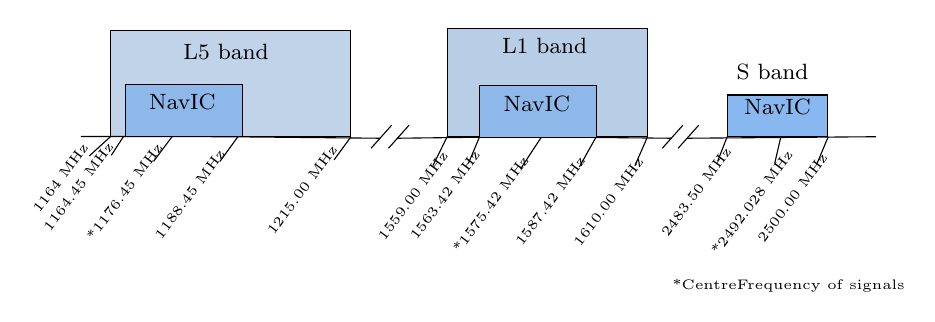
\begin{tikzpicture}[x=0.75pt,y=0.75pt,yscale=-1,xscale=1]
%uncomment if require: \path (0,471); %set diagram left start at 0, and has height of 471

%Shape: Rectangle [id:dp9517205987034671] 
\draw  [fill={rgb, 255:red, 192; green, 211; blue, 233 }  ,fill opacity=1 ] (92.53,176.6) -- (208.12,176.6) -- (208.12,227.79) -- (92.53,227.79) -- cycle ;
%Shape: Rectangle [id:dp3424557357689655] 
\draw  [fill={rgb, 255:red, 184; green, 205; blue, 230 }  ,fill opacity=1 ] (254.8,175.52) -- (351.33,175.52) -- (351.33,227.79) -- (254.8,227.79) -- cycle ;
%Shape: Rectangle [id:dp8560354037740456] 
\draw  [fill={rgb, 255:red, 137; green, 183; blue, 239 }  ,fill opacity=1 ] (389.7,207.67) -- (438,207.67) -- (438,227.79) -- (389.7,227.79) -- cycle ;
%Straight Lines [id:da4982550625943454] 
\draw    (78.33,227.67) -- (148.8,227.79) ;
%Straight Lines [id:da09038165069225701] 
\draw    (148.8,227.79) -- (222.43,228.52) ;
%Straight Lines [id:da6963693922945375] 
\draw    (230.82,228.52) -- (290.62,227.79) ;
%Straight Lines [id:da5101605840021868] 
\draw    (290.62,227.79) -- (362.75,228.52) ;
%Straight Lines [id:da4455724073590175] 
\draw    (218.13,233.34) -- (222.43,228.52) -- (228.04,222.24) ;
%Straight Lines [id:da44617587453109] 
\draw    (370.38,228.52) -- (461.33,227.79) ;
%Shape: Rectangle [id:dp9436860161134495] 
\draw  [fill={rgb, 255:red, 142; green, 184; blue, 233 }  ,fill opacity=1 ] (99.9,202.67) -- (156.33,202.67) -- (156.33,227.7) -- (99.9,227.7) -- cycle ;
%Straight Lines [id:da1306791733179924] 
\draw    (226.51,233.34) -- (230.82,228.52) -- (236.42,222.24) ;
%Straight Lines [id:da9755728827987384] 
\draw    (358.45,233.34) -- (362.75,228.52) -- (368.36,222.24) ;
%Straight Lines [id:da6153463426480046] 
\draw    (366.07,233.34) -- (370.38,228.52) -- (375.98,222.24) ;
%Straight Lines [id:da524212389543216] 
\draw    (92.53,227.79) -- (82.36,237.05) ;
%Straight Lines [id:da6359631954084011] 
\draw    (98.83,227.7) -- (92.93,236.8) ;
%Straight Lines [id:da4309637537474662] 
\draw    (122.33,227.67) -- (113.33,239.67) ;
%Straight Lines [id:da7084848716058743] 
\draw    (154.02,227.7) -- (145.34,239.67) ;
%Straight Lines [id:da9025278744467291] 
\draw    (208.45,227.79) -- (200.32,238.9) ;
%Straight Lines [id:da4288601859090342] 
\draw    (254.8,227.79) -- (247.94,241.67) ;
%Straight Lines [id:da6434353112428917] 
\draw    (270.26,228.16) -- (265,240.67) ;
%Straight Lines [id:da6934497348254585] 
\draw    (299.96,228.29) -- (290.19,243.19) ;
%Straight Lines [id:da08356280974055585] 
\draw    (326.33,228.29) -- (318.52,242.26) ;
%Straight Lines [id:da47170852835093413] 
\draw    (389.7,227.79) -- (385.12,239.51) ;
%Straight Lines [id:da39211419648473833] 
\draw    (415.47,228.16) -- (412.56,240.75) ;
%Straight Lines [id:da6629675504582904] 
\draw    (438.38,227.79) -- (433,240.67) ;
%Straight Lines [id:da16092426119270775] 
\draw    (351.33,227.79) -- (345.23,241.76) ;
%Shape: Rectangle [id:dp5224743842810824] 
\draw  [fill={rgb, 255:red, 142; green, 184; blue, 233 }  ,fill opacity=1 ] (270.26,203.12) -- (326.69,203.12) -- (326.69,228.16) -- (270.26,228.16) -- cycle ;

% Text Node
\draw (393.01,191.59) node [anchor=north west][inner sep=0.75pt]   [align=left] {{\footnotesize S band}};
% Text Node
\draw (396.7,208.67) node [anchor=north west][inner sep=0.75pt]   [align=left] {{\footnotesize NavIC}};
% Text Node
\draw (279.94,179.23) node [anchor=north west][inner sep=0.75pt]  [font=\footnotesize] [align=left] {L1 band};
% Text Node
%\draw (100.68,152.4) node [anchor=north west][inner sep=0.75pt]  [font=\scriptsize] [align=left] {ARNS / RNSS Band};
% Text Node
\draw (126.47,182.01) node [anchor=north west][inner sep=0.75pt]  [font=\footnotesize] [align=left] {L5 band};
% Text Node
\draw (109.89,206.05) node [anchor=north west][inner sep=0.75pt]   [align=left] {{\footnotesize NavIC}};
% Text Node
\draw (280.67,206.99) node [anchor=north west][inner sep=0.75pt]  [font=\normalsize] [align=left] {{\footnotesize NavIC}};
% Text Node
%\draw (252.7,152.4) node [anchor=north west][inner sep=0.75pt]  [font=\scriptsize] [align=left] {ARNS / RNSS Band};
% Text Node
%\draw (367.49,152.32) node [anchor=north west][inner sep=0.75pt]  [font=\scriptsize] [align=left] {RNSS/RDSS Band};
% Text Node
\draw (52.94,262.5) node [anchor=north west][inner sep=0.75pt]  [font=\scriptsize,rotate=-306.7] [align=left] {{\tiny 1164 MHz}};
% Text Node
\draw (58.07,271.48) node [anchor=north west][inner sep=0.75pt]  [font=\scriptsize,rotate=-306.7] [align=left] {{\tiny 1164.45 MHz}};
% Text Node
\draw (78.65,275.41) node [anchor=north west][inner sep=0.75pt]  [font=\scriptsize,rotate=-306.7] [align=left] {{\tiny *1176.45 MHz}};
% Text Node
\draw (111.71,275.12) node [anchor=north west][inner sep=0.75pt]  [font=\scriptsize,rotate=-306.7] [align=left] {{\tiny 1188.45 MHz}};
% Text Node
\draw (165.87,273.01) node [anchor=north west][inner sep=0.75pt]  [font=\scriptsize,rotate=-306.7] [align=left] {{\tiny 1215.00 MHz}};
% Text Node
\draw (219.28,275.78) node [anchor=north west][inner sep=0.75pt]  [font=\scriptsize,rotate=-306.7] [align=left] {{\tiny 1559.00 MHz}};
% Text Node
\draw (234.71,275.48) node [anchor=north west][inner sep=0.75pt]  [font=\scriptsize,rotate=-306.7] [align=left] {{\tiny 1563.42 MHz}};
% Text Node
\draw (255.1,281.42) node [anchor=north west][inner sep=0.75pt]  [font=\scriptsize,rotate=-306.7] [align=left] {{\tiny *1575.42 MHz}};
% Text Node
\draw (285.46,278.33) node [anchor=north west][inner sep=0.75pt]  [font=\scriptsize,rotate=-306.7] [align=left] {{\tiny 1587.42 MHz}};
% Text Node
\draw (313.45,278.62) node [anchor=north west][inner sep=0.75pt]  [font=\scriptsize,rotate=-306.7] [align=left] {{\tiny 1610.00 MHz}};
% Text Node
\draw (355.7,273.93) node [anchor=north west][inner sep=0.75pt]  [font=\scriptsize,rotate=-306.7] [align=left] {{\tiny 2483.50 MHz}};
% Text Node
\draw (379.59,282.47) node [anchor=north west][inner sep=0.75pt]  [font=\scriptsize,rotate=-306.7] [align=left] {{\tiny *2492.028 MHz}};
% Text Node
\draw (402.14,276.71) node [anchor=north west][inner sep=0.75pt]  [font=\scriptsize,rotate=-306.7] [align=left] {{\tiny 2500.00 MHz}};
% Text Node
\draw (362,295) node [anchor=north west][inner sep=0.75pt]  [font=\tiny] [align=left] {{\tiny *CentreFrequency of signals}};

\end{tikzpicture}

	\caption{Frequency bands of NavIC Signals}
	\label{figure:bandsfig}
	\end{figure}

\begin{table}[!ht]
	\small
	\centering
	%\subimport{table/}{table1.tex}
	%%%%%%%%%%%%%%%%%%%%%%%%%%%%%%%%%%%%%%%%%%%%%%%%%%%%%%%%%%%%%%%%%%%%%%
%%                                                                  %%
%%  This is the header of a LaTeX2e file exported from Gnumeric.    %%
%%                                                                  %%
%%  This file can be compiled as it stands or included in another   %%
%%  LaTeX document. The table is based on the longtable package so  %%
%%  the longtable options (headers, footers...) can be set in the   %%
%%  preamble section below (see PRAMBLE).                           %%
%%                                                                  %%
%%  To include the file in another, the following two lines must be %%
%%  in the including file:                                          %%
%%        \def\inputGnumericTable{}                                 %%
%%  at the beginning of the file and:                               %%
%%        \input{name-of-this-file.tex}                             %%
%%  where the table is to be placed. Note also that the including   %%
%%  file must use the following packages for the table to be        %%
%%  rendered correctly:                                             %%
%%    \usepackage[latin1]{inputenc}                                 %%
%%    \usepackage{color}                                            %%
%%    \usepackage{array}                                            %%
%%    \usepackage{longtable}                                        %%
%%    \usepackage{calc}                                             %%
%%    \usepackage{multirow}                                         %%
%%    \usepackage{hhline}                                           %%
%%    \usepackage{ifthen}                                           %%
%%  optionally (for landscape tables embedded in another document): %%
%%    \usepackage{lscape}                                           %%
%%                                                                  %%
%%%%%%%%%%%%%%%%%%%%%%%%%%%%%%%%%%%%%%%%%%%%%%%%%%%%%%%%%%%%%%%%%%%%%%



%%  This section checks if we are begin input into another file or  %%
%%  the file will be compiled alone. First use a macro taken from   %%
%%  the TeXbook ex 7.7 (suggestion of Han-Wen Nienhuys).            %%
\def\ifundefined#1{\expandafter\ifx\csname#1\endcsname\relax}


%%  Check for the \def token for inputed files. If it is not        %%
%%  defined, the file will be processed as a standalone and the     %%
%%  preamble will be used.                                          %%
\ifundefined{inputGnumericTable}

%%  We must be able to close or not the document at the end.        %%
	\def\gnumericTableEnd{\end{document}}


%%%%%%%%%%%%%%%%%%%%%%%%%%%%%%%%%%%%%%%%%%%%%%%%%%%%%%%%%%%%%%%%%%%%%%
%%                                                                  %%
%%  This is the PREAMBLE. Change these values to get the right      %%
%%  paper size and other niceties.                                  %%
%%                                                                  %%
%%%%%%%%%%%%%%%%%%%%%%%%%%%%%%%%%%%%%%%%%%%%%%%%%%%%%%%%%%%%%%%%%%%%%%

	\documentclass[12pt%
			  %,landscape%
                    ]{report}
       \usepackage[latin1]{inputenc}
       \usepackage{fullpage}
       \usepackage{color}
       \usepackage{array}
       \usepackage{longtable}
       \usepackage{calc}
       \usepackage{multirow}
       \usepackage{hhline}
       \usepackage{ifthen}

	\begin{document}


%%  End of the preamble for the standalone. The next section is for %%
%%  documents which are included into other LaTeX2e files.          %%
\else

%%  We are not a stand alone document. For a regular table, we will %%
%%  have no preamble and only define the closing to mean nothing.   %%
    \def\gnumericTableEnd{}

%%  If we want landscape mode in an embedded document, comment out  %%
%%  the line above and uncomment the two below. The table will      %%
%%  begin on a new page and run in landscape mode.                  %%
%       \def\gnumericTableEnd{\end{landscape}}
%       \begin{landscape}


%%  End of the else clause for this file being \input.              %%
\fi

%%%%%%%%%%%%%%%%%%%%%%%%%%%%%%%%%%%%%%%%%%%%%%%%%%%%%%%%%%%%%%%%%%%%%%
%%                                                                  %%
%%  The rest is the gnumeric table, except for the closing          %%
%%  statement. Changes below will alter the table's appearance.     %%
%%                                                                  %%
%%%%%%%%%%%%%%%%%%%%%%%%%%%%%%%%%%%%%%%%%%%%%%%%%%%%%%%%%%%%%%%%%%%%%%

\providecommand{\gnumericmathit}[1]{#1} 
%%  Uncomment the next line if you would like your numbers to be in %%
%%  italics if they are italizised in the gnumeric table.           %%
%\renewcommand{\gnumericmathit}[1]{\mathit{#1}}
\providecommand{\gnumericPB}[1]%
{\let\gnumericTemp=\\#1\let\\=\gnumericTemp\hspace{0pt}}
 \ifundefined{gnumericTableWidthDefined}
        \newlength{\gnumericTableWidth}
        \newlength{\gnumericTableWidthComplete}
        \newlength{\gnumericMultiRowLength}
        \global\def\gnumericTableWidthDefined{}
 \fi
%% The following setting protects this code from babel shorthands.  %%
 \ifthenelse{\isundefined{\languageshorthands}}{}{\languageshorthands{english}}
%%  The default table format retains the relative column widths of  %%
%%  gnumeric. They can easily be changed to c, r or l. In that case %%
%%  you may want to comment out the next line and uncomment the one %%
%%  thereafter                                                      %%
\providecommand\gnumbox{\makebox[0pt]}
%%\providecommand\gnumbox[1][]{\makebox}

%% to adjust positions in multirow situations                       %%
\setlength{\bigstrutjot}{\jot}
\setlength{\extrarowheight}{\doublerulesep}

%%  The \setlongtables command keeps column widths the same across  %%
%%  pages. Simply comment out next line for varying column widths.  %%
\setlongtables

\setlength\gnumericTableWidth{%
	53pt+%
	107pt+%
	65pt+%
	65pt+%
0pt}
\def\gumericNumCols{3}
\setlength\gnumericTableWidthComplete{\gnumericTableWidth+%
         \tabcolsep*\gumericNumCols*2+\arrayrulewidth*\gumericNumCols}
\ifthenelse{\lengthtest{\gnumericTableWidthComplete > \linewidth}}%
         {\def\gnumericScale{\ratio{\linewidth-%
                        \tabcolsep*\gumericNumCols*2-%
                        \arrayrulewidth*\gumericNumCols}%
{\gnumericTableWidth}}}%
{\def\gnumericScale{1}}

%%%%%%%%%%%%%%%%%%%%%%%%%%%%%%%%%%%%%%%%%%%%%%%%%%%%%%%%%%%%%%%%%%%%%%
%%                                                                  %%
%% The following are the widths of the various columns. We are      %%
%% defining them here because then they are easier to change.       %%
%% Depending on the cell formats we may use them more than once.    %%
%%                                                                  %%
%%%%%%%%%%%%%%%%%%%%%%%%%%%%%%%%%%%%%%%%%%%%%%%%%%%%%%%%%%%%%%%%%%%%%%

\ifthenelse{\isundefined{\gnumericColA}}{\newlength{\gnumericColA}}{}\settowidth{\gnumericColA}{\begin{tabular}{@{}p{40pt*\gnumericScale}@{}}x\end{tabular}}
\ifthenelse{\isundefined{\gnumericColB}}{\newlength{\gnumericColB}}{}\settowidth{\gnumericColB}{\begin{tabular}{@{}p{85pt*\gnumericScale}@{}}x\end{tabular}}
\ifthenelse{\isundefined{\gnumericColC}}{\newlength{\gnumericColC}}{}\settowidth{\gnumericColC}{\begin{tabular}{@{}p{60pt*\gnumericScale}@{}}x\end{tabular}}
\ifthenelse{\isundefined{\gnumericColD}}{\newlength{\gnumericColD}}{}\settowidth{\gnumericColD}{\begin{tabular}{@{}p{112pt*\gnumericScale}@{}}x\end{tabular}}
\begin{longtable}[c]{%
	b{\gnumericColA}%
	b{\gnumericColB}%
	b{\gnumericColC}%
	b{\gnumericColD}%
	}

%%%%%%%%%%%%%%%%%%%%%%%%%%%%%%%%%%%%%%%%%%%%%%%%%%%%%%%%%%%%%%%%%%%%%%
%%  The longtable options. (Caption, headers... see Goosens, p.124) %%
%	\caption{The Table Caption.}             \\	%
% \hline	% Across the top of the table.
%%  The rest of these options are table rows which are placed on    %%
%%  the first, last or every page. Use \multicolumn if you want.    %%

%%  Header for the first page.                                      %%
%	\multicolumn{3}{c}{The First Header} \\ \hline 
%	\multicolumn{1}{c}{colTag}	%Column 1
%	&\multicolumn{1}{c}{colTag}	%Column 2
%	&\multicolumn{1}{c}{colTag}	\\ \hline %Last column
%	\endfirsthead

%%  The running header definition.                                  %%
%	\hline
%	\multicolumn{3}{l}{\ldots\small\slshape continued} \\ \hline
%	\multicolumn{1}{c}{colTag}	%Column 1
%	&\multicolumn{1}{c}{colTag}	%Column 2
%	&\multicolumn{1}{c}{colTag}	\\ \hline %Last column
%	\endhead

%%  The running footer definition.                                  %%
%	\hline
%	\multicolumn{3}{r}{\small\slshape continued\ldots} \\
%	\endfoot

%%  The ending footer definition.                                   %%
%	\multicolumn{3}{c}{That's all folks} \\ \hline 
%	\endlastfoot
%%%%%%%%%%%%%%%%%%%%%%%%%%%%%%%%%%%%%%%%%%%%%%%%%%%%%%%%%%%%%%%%%%%%%%

\hhline{|-|-|-|-}
	 \multicolumn{1}{|p{\gnumericColA}|}%
	{\gnumericPB{\raggedright}\gnumbox[l]{Bands}}
	&\multicolumn{1}{p{\gnumericColB}|}%
	{\gnumericPB{\raggedright}\gnumbox[l]{Carrier Frequency}}
	&\multicolumn{1}{p{\gnumericColC}|}%
	{\gnumericPB{\raggedright}\gnumbox[l]{Bandwidth}}
	&\multicolumn{1}{p{\gnumericColD}|}%
	{\gnumericPB{\raggedright}\gnumbox[l]{Usage}}
\\
\hhline{|----|}
	 \multicolumn{1}{|p{\gnumericColA}|}%
	{\gnumericPB{\raggedright}\gnumbox[l]{L1}}
	&\multicolumn{1}{p{\gnumericColB}|}%
	{\gnumericPB{\raggedright}\gnumbox[l]{1575.42 Mhz}}
	&\multicolumn{1}{p{\gnumericColC}|}%
	{\gnumericPB{\raggedright}\gnumbox[l]{24 Mhz}}
	&\multicolumn{1}{p{\gnumericColD}|}%
	{\gnumericPB{\raggedright}\gnumbox[l]{for low power devices}}
\\
\hhline{|----|}
	 \multicolumn{1}{|p{\gnumericColA}|}%
	{\gnumericPB{\raggedright}\gnumbox[l]{L5}}
	&\multicolumn{1}{p{\gnumericColB}|}%
	{\gnumericPB{\raggedright}\gnumbox[l]{1176.45 Mhz}}
	&\multicolumn{1}{p{\gnumericColC}|}%
	{\gnumericPB{\raggedright}\gnumbox[l]{24 Mhz}}
	&\multicolumn{1}{p{\gnumericColD}|}%
	{\gnumericPB{\raggedright}\gnumbox[l]{navigation and positioning}}
\\
\hhline{|----|}
	 \multicolumn{1}{|p{\gnumericColA}|}%
	{\gnumericPB{\raggedright}\gnumbox[l]{S}}
	&\multicolumn{1}{p{\gnumericColB}|}%
	{\gnumericPB{\raggedright}\gnumbox[l]{2492.028 Mhz}}
	&\multicolumn{1}{p{\gnumericColC}|}%
	{\gnumericPB{\raggedright}\gnumbox[l]{16.5 Mhz}}
	&\multicolumn{1}{p{\gnumericColD}|}%
	{\gnumericPB{\raggedright}\gnumbox[l]{SBAS and messaging}}

\\
\hhline{|-|-|-|-|}
\end{longtable}

\ifthenelse{\isundefined{\languageshorthands}}{}{\languageshorthands{\languagename}}
\gnumericTableEnd

	\caption{NavIC frequency bands}
	\label{table:bands}
	\end{table}

\noindent Satellite communication utilizes multiple frequency bands to accommodate different types of communication services and addresses various technical considerations. Here are some reasons why multiple frequency bands are used in satellite communication:
\\
\\
\textbf{Spectrum Allocation:} The electromagnetic spectrum is divided into various frequency bands to allocate different services and applications. This division ensures that different systems can operate without interfering with each other. By utilizing multiple frequency bands, satellite communication can effectively coexist with other wireless services and minimize interference issues.
\\
\\
\textbf{Signal Propagation Characteristics:} Different frequency bands exhibit unique propagation characteristics. Lower frequency bands, such as L band, have better signal penetration through obstacles and are less affected by atmospheric conditions, making them suitable for applications where signal reliability is crucial. Higher frequency bands, such as Ku band or Ka band, offer larger bandwidths and higher data transmission rates, making them ideal for applications requiring high-speed data transfer.
\\
\\
\textbf{Bandwidth and Capacity:} Different frequency bands offer varying bandwidths, and by utilizing multiple bands, satellite communication systems can increase overall capacity. This allows for the simultaneous transmission of multiple signals, accommodating a wide range of services such as television broadcasting, voice communication, internet access, and data transfer.
\\
\\
\textbf{Frequency Reuse and Interference Mitigation:} Satellite systems employ frequency reuse techniques to maximize the utilization of the available frequency spectrum. By using different frequency bands, satellite operators can reuse frequencies in different geographical areas without causing interference. This allows for efficient utilization of the limited spectrum resources.
\\
\\
\textbf{Regulation and International Coordination:} The allocation and usage of frequency bands are regulated by international bodies and national spectrum management organizations. These regulations help ensure efficient spectrum utilization, prevent interference between different systems, and promote global coordination and compatibility of satellite communication services.
\\
\\
In summary, the use of multiple frequency bands in satellite communication enables efficient spectrum utilization, accommodates different services, and addresses various technical considerations such as signal propagation, bandwidth, capacity, and interference mitigation. By leveraging the advantages offered by different frequency ranges, satellite systems can provide reliable, high-speed communication services to a wide range of applications and users.

\noindent The seven satellites in the NavIC constellation so far use two frequencies for providing positioning data — the L5 and S bands. This was because India hadn't received the International Telecommunication Union authorisation for using the L1 and L2 frequency bands, which are widely used worldwide for navigation services. The new satellites NVS-01 onwards, meant to replace these satellites, will also have L1 band. L1 is an interoperable frequency and can be used across all chipsets(of mobile devices), provided they use our signal architecture.

\subsection{L-band}
The L band offers several advantages for wireless communication systems, including a balance between signal propagation characteristics and antenna size. It provides good signal penetration through various atmospheric conditions, vegetation, and even some obstacles. These properties make it suitable for applications such as satellite communication, navigation systems, and mobile networks.

\noindent Satellite communication is one of the significant applications of the L band. Satellites in geostationary orbits often utilize this frequency range for broadcasting television signals, as well as for maritime, navigation and aeronautical communications. The L band allows for reliable and efficient transmission over long distances, making it a valuable resource for global connectivity. Because of satellites’ increased use, number and size, congestion has become a serious issue in the lower frequency bands.

\noindent L1 and L5 are specific frequencies within the L band that are used in Global Navigation Satellite Systems (GNSS), such as GPS (Global Positioning System), NavIC and Galileo. These frequencies play a crucial role in providing accurate positioning, navigation, and timing information.
\subsubsection{L1} 
L1 refers to the first frequency within the L band used by GNSS. In NavIC, the L1 frequency is centered around $1575.42$ MHz. The L1 signal carries the primary navigation message and is used for standard positioning and timing applications. It is widely used in various sectors, including transportation, surveying, and consumer applications like personal navigation devices and smartphones.
\subsubsection{L5}
L5, on the other hand, is an additional frequency introduced in modernized GNSS systems like GPS and Galileo. In NavIC, the L5 frequency is centered around $1176.45$ MHz. It was introduced to provide improved accuracy, integrity, and resistance to interference. The L5 signal carries more precise and reliable positioning information, making it particularly useful in critical applications that require high levels of accuracy, such as aviation, surveying, and scientific research.
The L1 frequency offers broad coverage and compatibility with legacy systems, while the L5 frequency provides more precise positioning and improved resistance to interference. The combination of these frequencies allows for more reliable and accurate navigation solutions, benefiting a wide range of industries and applications.
\subsection{S-band} 
The S band is another frequency range within the electromagnetic spectrum, located between the L band and the C band. It spans a frequency range of approximately $2$ to $4$ GHz. In NavIC, S band frequency is centred around $2492.028$ MHz. The S band finds applications in various fields, including communication, radar systems, satellite broadcasting, and scientific research.
\\
One of the primary uses of the S band is in satellite communication. Satellites in geostationary orbits often utilize S band frequencies for uplink and downlink communication with ground stations. The S band provides a good balance between antenna size and data capacity, making it suitable for broadcasting television signals, voice communication, and data transmission. However, the higher frequency bands typically give access to wider bandwidths, but are also more susceptible to signal degradation due to ‘rain fade’ (the absorption of radio signals by atmospheric rain, snow or ice).

\section{NavIC Architecture}	
The NavIC architecture is as shown in Fig \ref{figs:archfig}. It mainly consists of 
\begin{enumerate}
	\item Space segment 
	\item Ground segment 
	\item User segment 
\end{enumerate}

	\begin{figure}[!ht]
	\centering
	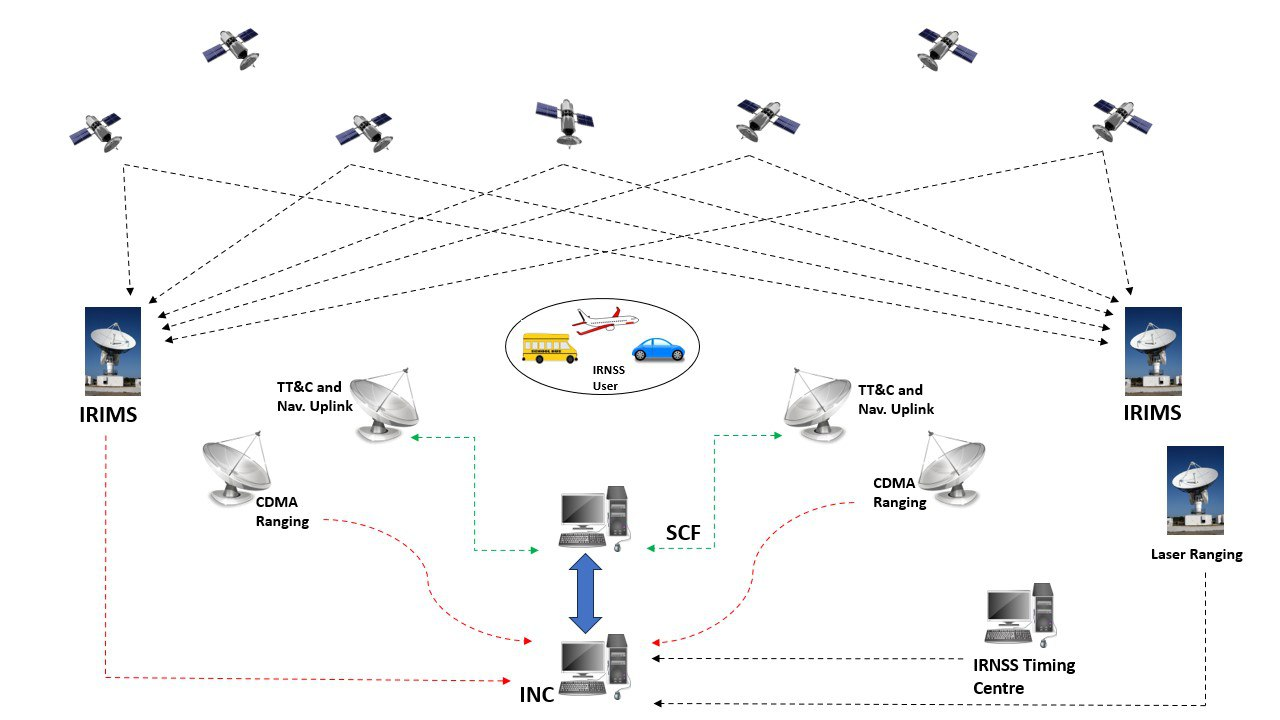
\includegraphics[width=\columnwidth]{figs/Architecture.jpg}
	\caption{NavIC Architecture}
	\label{figs:archfig}
	\end{figure}

\subsection{Space segment}
Space segment consists of a constellation of $7$ satellites. Three satellites of the constellation are placed in geostationary orbit, at $32.5^{\circ}$E, $83^{\circ}$E and $129.5^{\circ}$E respectively, and four satellites are placed in inclined geosynchronous orbit with equatorial crossing of $55^{\circ}$E and $111.75^{\circ}$E respectively, with inclination of $29^{\circ}$ (two satellites in each plane).

\subsection{Ground segment}
Ground segment takes care of operation and maintenance of the constellation. It consists of 
\begin{enumerate}
	\item ISRO Navigation Centre
	\item IRNSS Spacecraft Control Facility
	\item IRNSS Range and Integrity Monitoring Stations
	\item IRNSS Network Timing Centre
	\item IRNSS CDMA Ranging Stations
	\item Laser Ranging Stations
	\item Data Communication Network
\end{enumerate}

\subsection{User segment}
User segment consists of 
\begin{enumerate}
	\item A single frequency receiver having capability to receive SPS signal at either L1, L5 or S band frequency
	\item A multi-frequency receiver having capability to receive SPS signal at combination of L1, L5 and S band frequencies
	\item A multi-constellation receiver compatible with NavIC and other GNSS signals.
\end{enumerate}
\noindent The Figure\ref{figs:bandsfig} above specifies the radio frequency interface between space and user segments.

	\begin{figure}[!ht]
	\centering
	%\subimport{table/}{table1.tex}
	\tikzset{every picture/.style={line width=0.75pt}} %set default line width to 0.75pt        
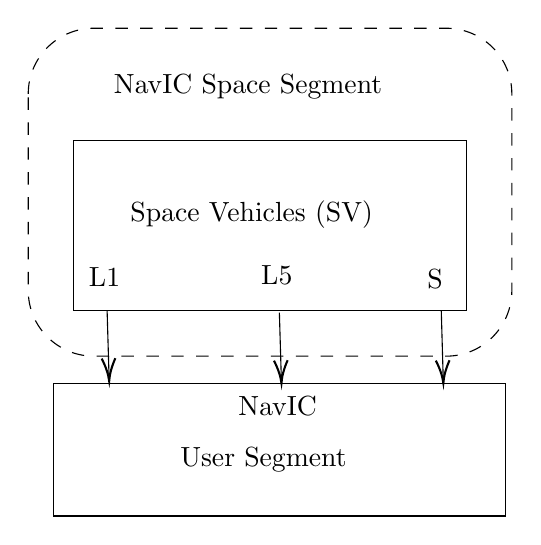
\begin{tikzpicture}[x=0.75pt,y=0.75pt,yscale=-1,xscale=1]
%uncomment if require: \path (0,406); %set diagram left start at 0, and has height of 406

%Shape: Rectangle [id:dp7411978076301706] 
\draw   (254,164) -- (443,164) -- (443,246) -- (254,246) -- cycle ;
%Straight Lines [id:da11098118487919195] 
\draw    (270,246) -- (270.94,278) ;
\draw [shift={(271,280)}, rotate = 268.32] [color={rgb, 255:red, 0; green, 0; blue, 0 }  ][line width=0.75]    (10.93,-3.29) .. controls (6.95,-1.4) and (3.31,-0.3) .. (0,0) .. controls (3.31,0.3) and (6.95,1.4) .. (10.93,3.29)   ;
%Shape: Rectangle [id:dp29610782491063636] 
\draw   (244,281) -- (462,281) -- (462,345) -- (244,345) -- cycle ;
%Straight Lines [id:da1330694648577655] 
\draw    (353,247) -- (353.94,279) ;
\draw [shift={(354,281)}, rotate = 268.32] [color={rgb, 255:red, 0; green, 0; blue, 0 }  ][line width=0.75]    (10.93,-3.29) .. controls (6.95,-1.4) and (3.31,-0.3) .. (0,0) .. controls (3.31,0.3) and (6.95,1.4) .. (10.93,3.29)   ;
%Straight Lines [id:da06268750746850027] 
\draw    (431,246) -- (431.94,279) ;
\draw [shift={(432,281)}, rotate = 268.36] [color={rgb, 255:red, 0; green, 0; blue, 0 }  ][line width=0.75]    (10.93,-3.29) .. controls (6.95,-1.4) and (3.31,-0.3) .. (0,0) .. controls (3.31,0.3) and (6.95,1.4) .. (10.93,3.29)   ;
%Rounded Rect [id:dp5981425610685245] 
\draw  [dash pattern={on 4.5pt off 4.5pt}] (232,141.6) .. controls (232,124.15) and (246.15,110) .. (263.6,110) -- (433.4,110) .. controls (450.85,110) and (465,124.15) .. (465,141.6) -- (465,236.4) .. controls (465,253.85) and (450.85,268) .. (433.4,268) -- (263.6,268) .. controls (246.15,268) and (232,253.85) .. (232,236.4) -- cycle ;

% Text Node
\draw (272,131) node [anchor=north west][inner sep=0.75pt]   [align=left] {NavIC Space Segment};
% Text Node
\draw (280,192) node [anchor=north west][inner sep=0.75pt]   [align=left] {Space Vehicles (SV)};
% Text Node
\draw (260,224) node [anchor=north west][inner sep=0.75pt]   [align=left] {L1};
% Text Node
\draw (343,223) node [anchor=north west][inner sep=0.75pt]   [align=left] {L5};
% Text Node
\draw (423,225) node [anchor=north west][inner sep=0.75pt]   [align=left] {S};
% Text Node
\draw (332,286) node [anchor=north west][inner sep=0.75pt]   [align=left] {NavIC};
% Text Node
\draw (304,311) node [anchor=north west][inner sep=0.75pt]   [align=left] {User Segment};

\end{tikzpicture}

	\caption{the NavIC bands segment blocks}
	\label{figs:bandsfig}
	\end{figure}

\section{NavIC Services}
The NavIC provides basically two types of services:
	\begin{enumerate}
	\item Standard Positioning Service (SPS)
	\item Restricted Service (RS)
	\end{enumerate}
Both SPS and RS signals contain ranging codes that allow receivers to compute their travelling time from satellite to receiver, along with navigation data, in order to know the satellite’s position at any time. 
\subsection{Standard Positioning Service (SPS)}
	It is available to all civilian users free of charge and provides positioning, navigation, and timing information with a moderate level of accuracy. The SPS signals in NavIC primarily operate in the L5 and S frequency bands.
\subsection{Restricted Service (RS)}
The RS is intended for authorized users and offers enhanced accuracy, integrity, and availability compared to the SPS signals. The RS signals in NavIC operate in both the L5 and S bands and broadcast through a phased array antenna to keep required coverage and signal strength. 
\let\cleardoublepage\clearpage  %to remove blank page
%\end{document}

\chapter{Navigation Data}

Navigation data in satellite communication refers to the crucial information transmitted between satellites and ground-based receivers to facilitate accurate positioning and navigation. It includes data related to satellite orbits, precise timing, and other parameters necessary for determining the satellite's position relative to the Earth's surface.
\section{Frame structure}
The NavIC L1 Master Frame is of $1800$ symbols long made of $3$ subframes. Subframe $1$ consists of $52$ symbols, Subframe $2$ is composed of 1$200$ symbols, and Subframe$3$ is comprised of $548$ symbols,The master frame structure is shown in figure \ref{fig:master_frame}


\begin{figure}[ht]
\centering
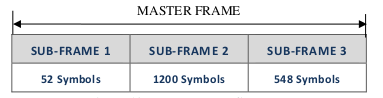
\includegraphics[width=0.8\columnwidth]{figs/master_frame.png}
\centering
\captionsetup{justification=centering}
\caption{Master Frame Structure}
\label{fig:master_frame}
\end{figure}


The Time of Interval (TOI)is transmitted in Subframe 1 is shown in figure \ref{fig:subframe1}. Subframe $2$ as shown in figure \ref{fig:subframe2}, transmitting the primary navigation parameters, and Subframe $3$ is shown in figure \ref{fig:subframe3}responsible for transmitting secondary navigation parameters.The secondary navigation parameters are transmitted in message format.It identifies the message types that the NavIC satellites will transmit. Provision exists to define new messages for future requirements in NavIC. Each message is identified by a unique message identifier.
 


\begin{figure}[ht]
\centering
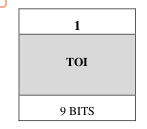
\includegraphics[width=0.4\columnwidth]{figs/subframe1.png}
\centering
\captionsetup{justification=centering}
\caption{ Sub-frame 1 Layout}
\label{fig:subframe1}
\end{figure}

\begin{figure}[ht]
\centering
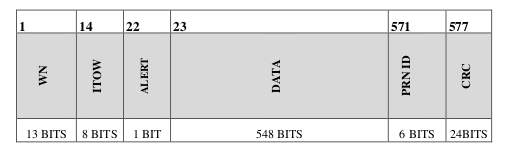
\includegraphics[width=0.8\columnwidth]{figs/subframe2.png}
\centering
\captionsetup{justification=centering}
\caption{Sub-frame 2 Layout}
\label{fig:subframe2}
\end{figure}

\begin{figure}[ht]
\centering
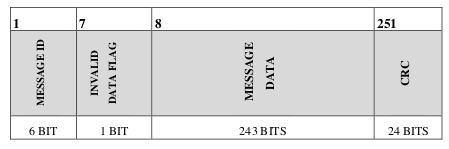
\includegraphics[width=0.8\columnwidth]{figs/subframe3.png}
\centering
\captionsetup{justification=centering}
\caption{Sub-frame 3 Layout}
\label{fig:subframe3}
\end{figure}
\subsection{L1 SPS DATA STRUCTURE}
The NavIC Signal-In-Space transmits navigation message data through the SPS service, in the L1 band. The sub-frame structure is shown in Figure \ref{fig: SPS_Structure}
\begin{figure}[ht]
\centering
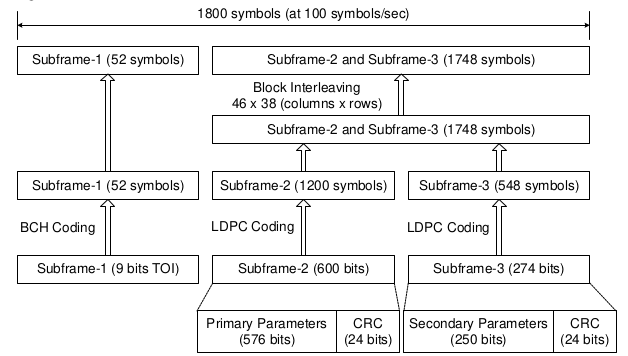
\includegraphics[width=0.8\columnwidth]{figs/SPS_Structure.png}
\centering
\captionsetup{justification=centering}
\caption{NavIC L1 SPS Subframe Structure}
\label{fig: SPS_Structure}
\end{figure}

\noindent The 600 bits of subframe $2$ and $274$ bits of subframe $3$ are Low Density Parity Check (LDPC) Forward Error Correction (FEC) encoded and interleaved as shown in Figure \ref{fig: SPS_Structure}. Subframe $2$ and subframe $3$ are separately encoded using rate $\frac{1}{2}$ Quasi Cyclic LDPC codes.
Subframe $1$ consists of $9$ bits that are Bose, Chaudhuri, and Hocquenghem (BCH) encoded.
Subframe $2$ has a total of $600$ bits, comprising $576$ bits for primary navigation parameters and $24$ bits for CRC.
Subframe $3$ contains a total of $274$ bits, with $250$ bits for secondary navigation parameters and $24$ bits for CRC.
sAs a result of rate $\frac{1}{2}$ Quasi Cyclic LDPC encoding, there are $1200$ symbols (coded bits) for subframe $2$ and $548$ symbols for subframe $3$, as described in Figure \ref{fig: SPS_Structure}.

\section{Cyclic Redundancy Check(CRC)}
The parity coding of data signal follows $24$Q polynomial for each subframe. $24$ bits of CRC parity will provide protection against burst as well as random errors with undetected error probability of $2^{-24}$ for all channel bit error probabilities $0.5$.
\begin{equation}
    g(X) = \sum_{i = 0}^{24}g_{i}X^i\;\; 
\end{equation}

    $g_{i}=1$; for $i = 0,1,3,4,5,6,7,10,11,14,17,18,23,24$ \\
          = 0 otherwise

\let\cleardoublepage\clearpage

\chapter{Simulation Approach}
The NavIC simulator approach is as shown in figure \ref{fig:sim_flow}.  

\begin{figure}[ht]
\centering
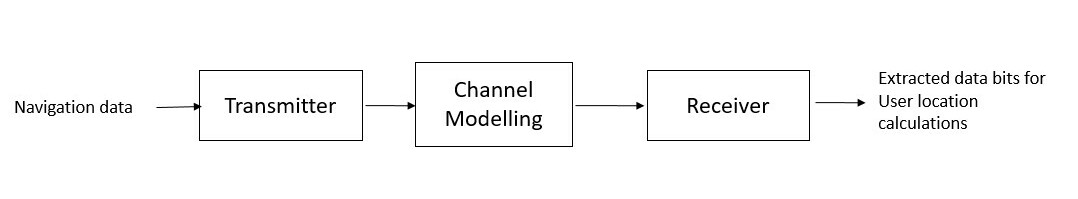
\includegraphics[width=1\columnwidth]{figs/simulation_overview.jpg}
\centering
\captionsetup{justification=centering}
\caption{Transmitter Block diagram}
\label{fig:sim_flow}
\end{figure}


Navigation data is randomly generated and subframes and master frames are created as per the frame structure described earlier. The transmitter module creates the required baseband signal as per the modulation scheme, with relevant channel encosing schemes. Channel modelling module adds various modelling parameteers and AWGN noise to the baseband signals for different satellites, forming a composite signal. The receiver module receives the composite signal, processes it to extract the navigation data, that was originally sent.  

\let\cleardoublepage\clearpage

\chapter{Transmitter}
The NavIC transmitter is simulated to send baseband signal to the channel as shown in Fig \ref{fig:trans_flow}. 

\begin{figure}[ht]
\centering
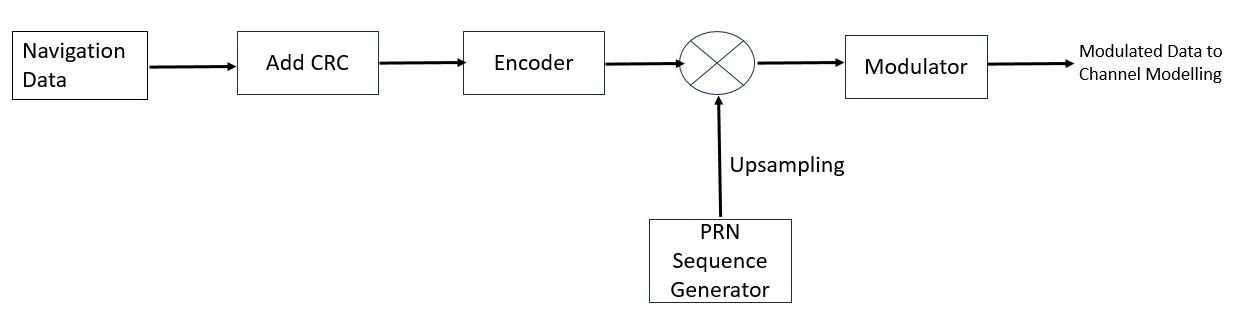
\includegraphics[width=1\columnwidth]{figs/trans_flow.jpg}
\centering
\captionsetup{justification=centering}
\caption{Transmitter Block diagram}
\label{fig:trans_flow}
\end{figure}

\section{Encoding}

\subsection{BCH Coding}

To transmit nine bits of Time of Interval (TOI) data, we employ BCH $(52, 9)$ coding. The generator polynomial used in this encoding process is $1767$ in octal notation. This coding scheme is illustrated conceptually in Figure~\ref{fig:generator} below, utilizing a 9-stage linear shift register generator.

\begin{figure}[ht]
    \centering
    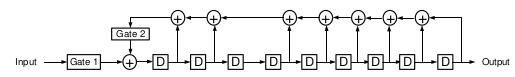
\includegraphics[width=1.05\columnwidth]{figs/bch.png}
    \caption{Diagram of the BCH Encoder Circuit}
    \label{fig:generator}
\end{figure}

\noindent\textbf{Encoding Process}

\noindent Load TOI data bits $1$ to $9$ into the generator, starting with the Most Significant Bit (MSB).Shift the loaded data $52$ times through the generator to generate $52$ encoded symbols.The BCH $(n, k)$ encoders are realized using $k$-stage registers as illustrated in Figure~\ref{fig:generator}. During encoding, Gate $1$ is closed for the initial $k$ clock periods and then disconnected. Likewise, Gate $2$ is disconnected during the first $k$ periods and then closed.



\begin{table}[h]
\centering
\caption{Generator Polynomials of BCH Encoders}
\label{table:generator_polynomials}
\begin{tabular}{|l|lll|l|}
\hline
\multirow{2}{*}{BCH Code} & \multicolumn{3}{c|}{Encoding Characteristics} & \multirow{2}{*}{Generator Polynomials (g(x))} \\
\cline{2-4}
& $n$ & $k$ & $d_{\text{min}}$ & \\
\hline
(52, 9) & 52 & 9 & 20 & $x^9 + x^8 + x^7 + x^6 + x^5 + x^4 + x^2 + x + 1$ \\
\hline
\end{tabular}
\end{table}

\subsection{LDPC}


\noindent The LDPC (Low-Density Parity-Check) encoder structure is based on a parity-check matrix $H(m, n)$ consisting of $m$ rows and $n$ columns. Specifically, for subframe-2, $m = 600$ and $n = 1200$, and for subframe-3, $m = 274$ and $n = 548$ are selected.

\noindent The LDPC matrix $H$ is assumed to be in an approximate lower triangular form with a dual diagonal structure. Matrix $H(m, n)$ is further decomposed into six submatrices: $A$, $B$, $T$, $C$, $D$, and $E$, as illustrated in Figure~\ref{fig:ldpc-structure} below.

\begin{figure}[ht]
\centering
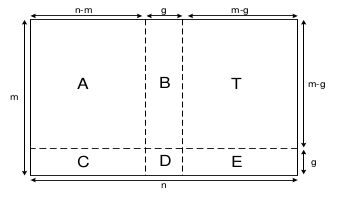
\includegraphics[width=1\columnwidth]{figs/ldpc.png}    
\caption{LDPC Matrix Structure}
\label{fig:ldpc-structure}
\end{figure}

\noindent Each element of matrix $H(m, n)$ takes on either the value $"0"$ or $"1"$.The inverse of matrix $T$, denoted as $T^{-1}$, is not included in this document. However, it is worth noting that since $T$ is a lower triangular matrix, its inverse can be readily identified.

For a rate $1/2$ LDPC encoder, the encoding process utilizes the matrices $A$, $B$, $T$, $C$, $D$, and $E$ to generate the encoded symbols based on the following algorithm:
\begin{align}
p_1^t &= -\varphi^{-1} (-E \cdot T^{-1} \cdot A + C) \cdot s^t \\
p_2^t &= -T^{-1} (A \cdot s^t + B \cdot p_1^t)
\end{align}


\noindent Where:
\begin{align*}
\varphi &= -E \cdot T^{-1} \cdot B + D \\
s &= \text{subframe 2 and subframe 3 data} \\
x_t &\text{ indicates transpose} \\
\end{align*}

\noindent The elements of matrices $p_1$ and $p_2$ are modulo 2 numbers.

\noindent The encoded symbols for broadcast are composed of $(s, p_1, p_2)$, where $s$ represents the systematic portion of the codeword, and $\{p_1, p_2\}$ constitute the combined parity bits.


\subsection{Interleaving}
\noindent Any burst errors during the data transmission can be corrected by interleaving. In matrix interleaving, input symbols are filled into a matrix column-wise and read at the output row-wise. This will spread the burst error, if any, during the transmission.The 1748 symbols of LDPC encoded navigation data of subframe-2 and subframe-3 are interleaved using a block interleaver with $n$ columns and $k$ rows. Data is written in columns and then read in rows. The Table \ref{tab:interleaving} below indicates the interleaving mechanism.

\begin{table}[ht]
\centering
\begin{tabular}{|l|l|}
\hline
\textbf{Parameter} & \textbf{Arrangement} \\
\hline
Block Interleaver size & 1748 \\
\hline
Block Interleaver Dimensions (n columns x k rows) & 46 x 38 \\
\hline
\end{tabular}
\caption{Interleaving Parameters}
\label{tab:interleaving}
\end{table}



\subsection{PRN codes for SPS}

\noindent The NavIC L1 signal utilizes a family of Interleaved Z4 – Linear (IZ4) PRN spreading codes implemented using coupled shift registers. The PRN code has a length of 10230 chips with a code period of 10 ms in both data and pilot channels. Furthermore, the pilot channel incorporates a secondary overlay code with a length of 1800 and a period of 18 s. Importantly, the pilot and data signals are designed to be orthogonal.
The IZ4 family of spreading codes has been found to deliver superior or equivalent performance compared to the PRN code families employed by GPS and BeiDou in the L1 band. Moreover, the resources required for implementing the code generator are of the same order as Weil codes.


\begin{figure}[ht]
\centering
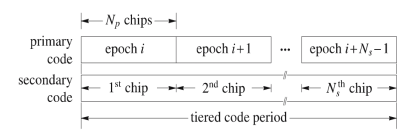
\includegraphics[width=\columnwidth]{figs/Tiered_code.png}
\centering
\captionsetup{justification=centering}
\caption{Tiered code structure and timing relationship between primary and secondary codes}
\label{fig:R0_IZ4}
\end{figure}



\begin{table}[h]
%\centering
\small
% Contents of table1.tex
%\begin{tabular}{|c|c|c|c|c|c|c|}
\begin{tabular}{|c|p{1.5cm}|p{1.3cm}|p{1.5cm}|p{1.5cm}|p{1.5cm}|p{1.5cm}|}
\hline
\textbf{Component} & \textbf{Primary Code Type} & \textbf{Primary Code Length} & \textbf{Primary Code Period (msec)} & \textbf{Secondary or Overlay Code Type} & \textbf{Secondary or Overlay Code Length} & \textbf{Secondary or Overlay Code Period (msec)} \\
\hline
L1 Data (L1D i (t)) & Z4–linear (IZ4) & 10230 & 10 & - & - & - \\
\hline
L1 Pilot (L1P i (t)) & Interleaved Z4–linear (IZ4) & 10230 & 10 & Truncated Z4-linear sequences & 1800 & 18000 \\
\hline
\end{tabular}

\vspace{3mm}
\caption{Characteristics of the L1 ranging codes}
\label{table:L1_ranging}
\end{table}

\subsubsection{Code Generator Architecture for primary L1 Pilot and L1 Data PRN Code}

\noindent The IZ4 ranging code generator comprises the following principal components:

\begin{enumerate}
    \item {Shift Registers R0 and R1:} These are two fifty-five tap binary shift registers.
    \item {Shift Register C:} This is a single, five-tap, binary, pure-cycling shift register.
\end{enumerate}

\textbf{Code Generation}

\noindent The IZ4 code is generated as the chip-by-chip modulo-2 sum of the synchronized output of Shift Register C and Register R1. Specifically, it is computed using the following equation:
\begin{align}
IZ4(t) = C(t, 0) \oplus R1(t, 0)
\label{eq:iz4} 
\end{align}
\noindent In this equation $C(t, 0)$ represents the first tap of Register C at time $t$, abbreviated as $C(0)$.
$R1(t, 0)$ represents the contents of the first tap of Register R1 at time $t$, abbreviated as $R1(0)$.
It's important to note that all three registers are synchronized with respect to each other, ensuring proper code generation.
It's important to note that all three registers are synchronized with respect to each other, ensuring proper code generation.

\begin{figure}[ht]
\centering
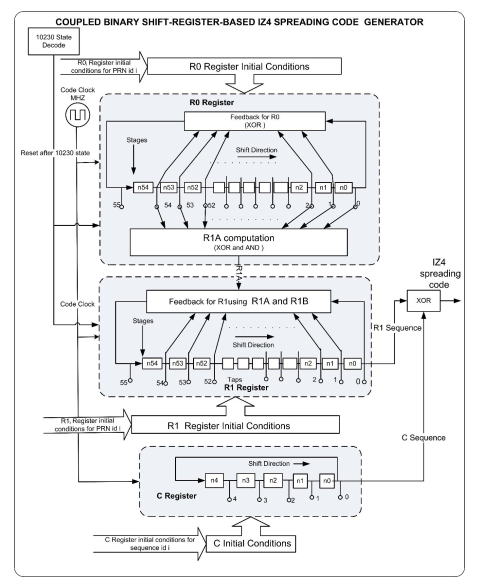
\includegraphics[width=0.8\columnwidth]{figs/IZ4_BCH.png}
\centering
\captionsetup{justification=centering}
\caption{Functional Description of IZ4 Sequence generation using Binary shift registers.}
\label{fig:IZ4_BCH}
\end{figure}

\noindent Functional description of each register involved in the IZ4 code generation process:

\subsubsection{Shift Register R0}

\noindent A fifty-five tap long $R0$ shift register is the first component.This register generates binary codes with a period of $10230$, shifting its contents at each clock cycle. The register's initial state is determined by stored initial conditions. It produces a binary code sequence with a $10230$-chip period, resetting after 10230 cycles. Feedback operations are governed by a feedback polynomial, with the output fed back to the $55^{th}$ tap. The first tap,$ R0(0)$, provides the component code output. In this process, seven out of $55$ taps are employed, following the equation: 

\begin{equation}
R0(54) = R0(50) \oplus R0(45) \oplus R0(40) \oplus R0(20) \oplus R0(10) \oplus R0(5) \oplus R0(0) 
\label{eq:R0(54)} 
\end{equation}

\begin{figure}[ht]
\centering
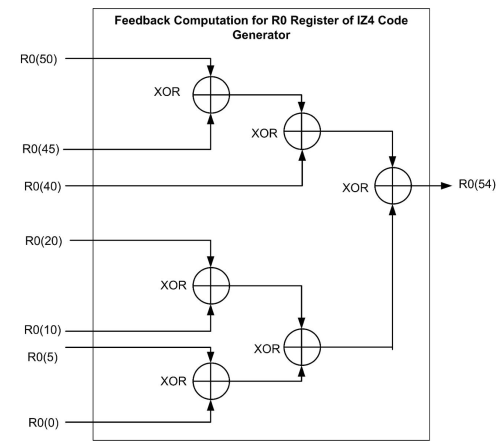
\includegraphics[width=0.8\columnwidth]{figs/R0_IZ4.png}
\centering
\captionsetup{justification=centering}
\caption{Feedback logic used to generate the linear feedback to Register R0 for IZ4 codes}
\label{fig:R0_IZ4}
\end{figure}
\noindent The feedback logic, illustrating inputs representing tap contents at time $(t)$ and output corresponding to the 55th tap at $(t+1)$, is depicted in Figure \ref{fig:R0_IZ4}.

\subsubsection{Shift Register R1}

\noindent The shift register \(R1\), consisting of fifty-five taps, serves as the source for generating the second component of the IZ4 ranging code. Similar to \(R0\), it operates by producing a binary code with a period of 10230 through content shifts at each clock cycle. The initial state of \(R1\) is determined by stored initial conditions, and it resets after 10230 clock cycles. The output originates from the first tap.

\noindent Feedback to \(R1\) encompasses both \(R1A\) and \(R1B\) components, computed as functions of the taps from both \(R0\) and \(R1\). The feedback to \(R1\) is the modulo-2 sum of \(R1A\) and \(R1B\).

Specifically, three sub-components, \(\sigma_2A\), \(\sigma_2B\), and \(\sigma_2C\), which depend on the tap contents of \(R0\), contribute to the computation of \(R1A\) as per the following equations:

\begin{equation}
\sigma_2A = [R0(50) \oplus R0(45) \oplus R0(40)] \text{ AND } [R0(20) \oplus R0(10) \oplus R0(5) \oplus R0(0)] 
\label{eq:sigma_2A } 
\end{equation}
\begin{equation}
\sigma_2B = ([R0(50) \oplus R0(45)] \text{ AND } R0(40)) \oplus  ([R0(20) \oplus R0(10)] \text{ AND }[R0(5) \oplus R0(0)]) 
\label{eq:sigma_2B } 
\end{equation}
\begin{equation}
\label{eq:sigma_2c} 
\sigma_2C = [R0(50) \text{ AND } R0(45)] \oplus ([R0(20) \text{ AND } \\ R0(10)]\oplus  [R0(5) \text{ AND }R0(0)])  
\end{equation}
\begin{equation}
\label{eq:sigma_2} 
\sigma_2 = \sigma_2A \oplus \sigma_2B \oplus \sigma_2C
\end{equation}
\begin{equation}
\label{eq:R1A} 
R1A = \sigma_2 \oplus [R0(40) \oplus R0(35) \oplus R0(30) \oplus R0(25) \oplus R0(15) \oplus R0(0)]
\end{equation}
\begin{equation}
\label{eq:R1B} 
R1B = R1(50) \oplus R1(45) \oplus R1(40) \oplus R1(20) \oplus R1(10) \oplus R1(5) \oplus R1(0)
\end{equation}
\begin{equation}
\label{eq:R154} 
R1(54) = R1A \oplus R1B
\end{equation}

In equations \ref{eq:sigma_2A } through \ref{eq:R1B}, all quantities represent contents or functions of register contents at time \(t\). Equation \ref{eq:R154} computes \(R1(54)\) at time \(t+1\) based on the quantities on the right side at time \(t\). All registers initialize with initial conditions at \(t=0\).
Implementation of the feedback computation for Shift Register \(R1\), where \(R1A\) and \(R1B\) are computed at time \(t\), and \(R1(54)\) refers to the contents \(R1(t+1,54)\) at time \(t+1\) of the 55th tap of Register \(R1\).

\begin{figure}[h]
    \centering
    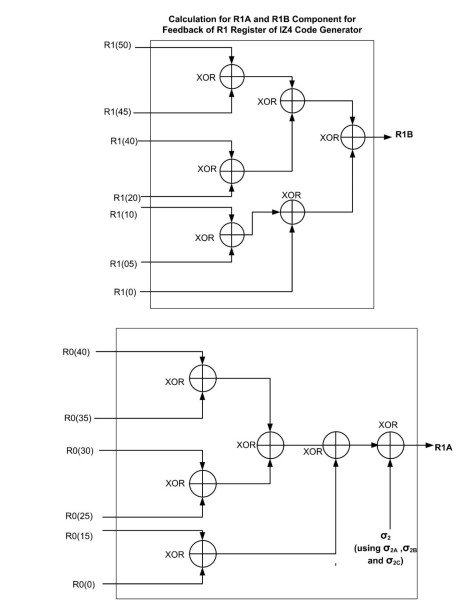
\includegraphics[width=\columnwidth]{figs/fig8.png}
    \captionsetup{justification=centering}
    \caption{Feedback Computation for R0 and R1A Determination for Overlay Codes}
    \label{fig:R0overlay}
\end{figure}

\begin{figure}[h]
    \centering
    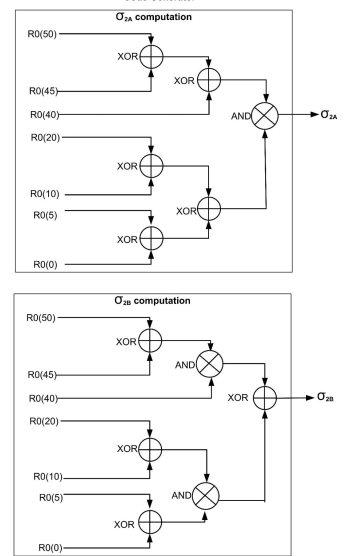
\includegraphics[width=\columnwidth]{figs/fig9.png}
    \captionsetup{justification=centering}
     \caption{$sigma2A$and $sigma2B$ Computation for R1A Determination for Primary IZ4 Codes}
    \label{fig:sigma2A_and_sigma2B_computation}
\end{figure}

\begin{figure}[h]
    \centering
    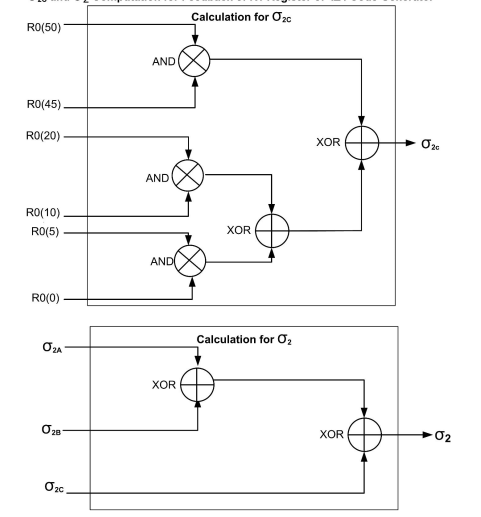
\includegraphics[width=\columnwidth]{figs/fig10.png}
    \captionsetup{justification=centering}
    \caption{$sigma2C$and $sigma2$ Computation for R1A Determination for Primary IZ4 Codes}
    \label{fig:sigma2C_and_sigma2_computation}
\end{figure}

\begin{figure}[h]
    \centering
    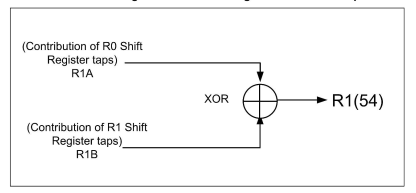
\includegraphics[width=\columnwidth]{figs/fig11.png}
    \captionsetup{justification=centering}
    \caption{R1 Feedback Computation Using R1 and R0 Shift Register Taps for Primary IZ4 Codes}
    \label{fig:R1Feedback}
\end{figure}





\subsubsection{Initial conditions for Shift Registers R0, R1 and C}
Each R0 and R1 component code generator uses 55 bits of unique initial conditions stored in memory.Shift Register C is a 5-tap pure-cycling register, where the first tap's output, denoted as C(0), is looped back as input to the fifth tap. C(0) is XORed with the output of the R1 shift register on a chip-by-chip basis to produce the IZ4 code. Initial five-bit conditions for Register C are provided in Tables 7 and 8, corresponding to each PRN code.
\subsection{Secondary Overlay Code Generator \\Architecture}
The secondary or overlay codes linked to each L1 pilot primary code have a length of 1800 chips. These overlay codes are independently synchronized in time and have a duration of 18 seconds, operating at a rate of 100 bps. The 1800-chip overlay codes are produced by cyclically cycling the Z4-linear codes, which have a period of 2046. The generation process for overlay codes resembles that of primary IZ4 codes. To generate overlay codes, two ten-tap shift registers, denoted as R0 and R1, are utilized with specific feedback polynomials. Unlike primary code generation, the C register is not necessary for the generation of overlay codes.

\begin{equation}
R0(9) = R0(5) \oplus R0(2) \oplus R0(1) \oplus R0(0) 
\end{equation}
\begin{equation}
\sigma_{2A} = [R0(5) \oplus R0(2)] \text{ AND } [R0(1) \oplus R0(0)]
\end{equation}
\begin{equation}
\sigma_{2B} = [R0(5) \text{ AND } R0(2)] \oplus [R0(1) \text{ AND } R0(0)] 
\end{equation}
\begin{equation}
R1A = \sigma_2 \oplus R0(6) \oplus R0(3) \oplus R0(2) \oplus R0(0) 
\end{equation}
\begin{equation}
R1B = R1(5) \oplus R1(2) \oplus R1(1) \oplus R1(0) 
\end{equation}
\begin{equation}
R1(9) = R1A \oplus R1B
\end{equation}


\begin{figure}[ht]
\centering
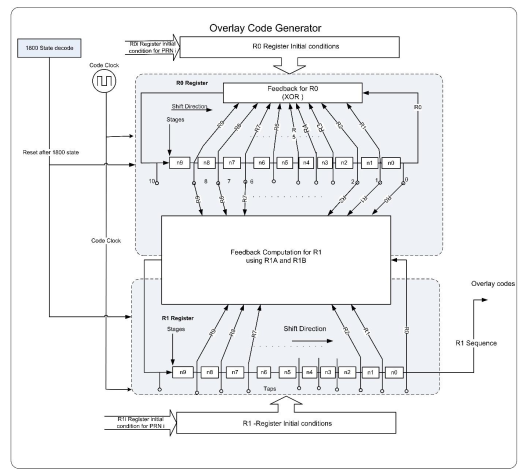
\includegraphics[width=\columnwidth]{figs/overlay.png}
\centering
\captionsetup{justification=centering}
\caption{Block Diagram of overlay sequence generator}
\label{fig:overlay}
\end{figure}

\begin{figure}[h]
    \centering
    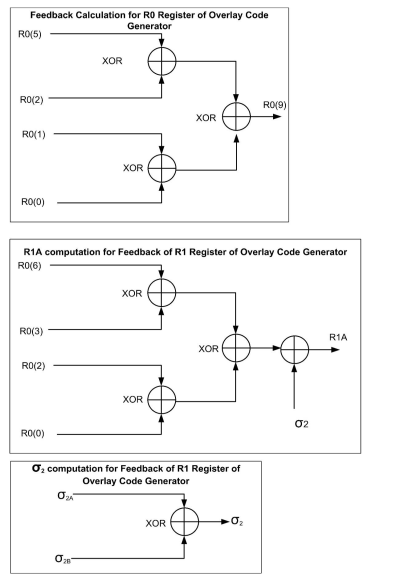
\includegraphics[width=\columnwidth]{figs/fig13.png}
    \captionsetup{justification=centering}
    \caption{Feedback Computation for R0 and R1A Determination for Overlay Codes}
    \label{fig:R0overlay}
\end{figure}

\begin{figure}[h]
    \centering
    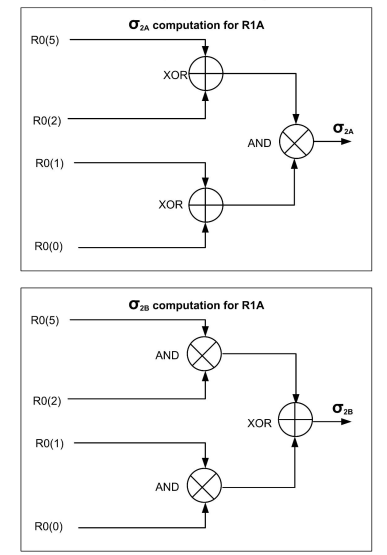
\includegraphics[width=\columnwidth]{figs/fig14.png}
    \captionsetup{justification=centering}
    \caption{$\sigma2A$ and $\sigma2B$ Computation for Overlay Codes}
    \label{fig:sigma2Boverlay}
\end{figure}

\begin{figure}[h]
    \centering
    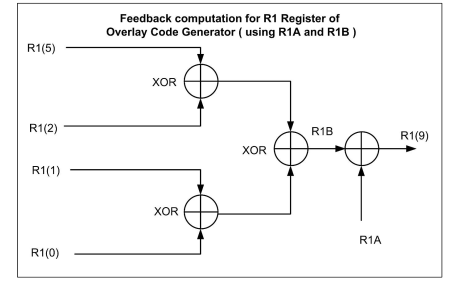
\includegraphics[width=\columnwidth]{figs/fig15.png}
    \captionsetup{justification=centering}
    \caption{R1 Register Feedback Computation for Overlay Codes}
    \label{fig:R1overlay}
\end{figure}

In Figures \ref{fig:R0overlay},\ref{fig:sigma2Boverlay}, and \ref{fig:R1overlay} below, the feedback computation process for $R_0$ and $R_1$ shift registers for overlay codes is explained. Figure \ref{fig:R0overlay} demonstrates how the feedback for Register $R_0$ is performed, along with the computation of certain components of the feedback for Register $R_1$. The output of Register $R_1$ corresponds to the overlay code. Quantities shown on the left, such as $R_0(5)$ in the topmost sub-figure of Figure~\ref{fig:R0overlay}, represent the contents of the respective registers at time $t$, while the quantity $R_0(9)$ on the opposite side represents the contents of $R_0$ at time $t+1$ for position 9.
\newpage

\section{Modulation}

\subsection{Standard Positioning Service}
\noindent The SPS signal is modulated using Synthesized Binary Offset Carrier (SBOC) in L1 band and BPSK in L5 and  S bands.
\subsection{Baseband Modulation}
\noindent SBOC modulation contains  BOC(1,1) and BOC(6,1) components in both data signal  and pilot signals.  In this scheme, the data channel's BOC(1,1), the pilot channel's BOC(1,1), and the pilot channel's BOC(6,1) components are interplexed to create the data channel's BOC(6,1) component.  Data and pilot signals are quadrature multiplexed, with $41.82\%$ power to data and $58.18\%$ to pilot, ensuring constant envelope modulation for MBOC.
\subsubsection{Mathematical Equations}
\noindent The mathematical representation of baseband navigation signals is as follows:

\textbf{Pilot Signal:}
\begin{equation}
S_{p,a}(t) = \sum_{i=-\infty}^{\infty} C_p(|i|L_p) \cdot \text{rect}_{T_{c,p}} \left( t - iT_{c,p}\right) \cdot s_{c,p,a}(t, 0)
\label{eq:sp_a}
\end{equation}

\begin{equation}
S_{p,b}(t) = \sum_{i=-\infty}^{\infty} C_p(|i|L_p) \cdot \text{rect}_{T_{c,p}}  \left( {t - iT_{c,p}}\right) \cdot sc_{p,b}(t, 0)
\label{eq:sp_b}
\end{equation}

\noindent The sub-carrier is defined as:

\begin{equation}
sc_{p,x}(t, \varphi) = \text{sgn}[\sin(2\pi f_{sc,x^t} + \varphi)]
\label{eq:sub_carrier}
\end{equation}

\noindent Ranging code $C_p$, defined in equations \eqref{eq:sp_a} and \eqref{eq:sp_b}, includes primary code and secondary overlay code.


\textbf{Data Signal:}

\begin{equation}
S_{d,a}(t) = \sum_{i=-\infty}^{\infty} C_d(|i|_{L_d}  ) \cdot d_d([i]_{CD_d}) \cdot \text{rect} _{T_{c,d}} \left({t - iT_{c,d}}\right) \cdot sc_{d,a}(t, 0)
\label{eq:signal_da}
\end{equation}

\noindent The sub-carrier is defined as:

\begin{equation}
sc_{d,x}(t, \varphi) = \text{sgn}[\sin(2\pi f_{sc,x^t} + \varphi)]
\label{eq:subcarrier_dc_x}
\end{equation}
\noindent The subcarrier signals are sinBOC. Hence, the subcarrier phase $\varphi=0$.

\noindent The interplexed component $(S_{d,b}(t)$ is given by:
\begin{equation}
S_{d,b}(t) = \sum_{i=-\infty}^{\infty} C_d(|i|L_d) \cdot d_d([i]C_{D_d}) \cdot \text{rect}_{T_{c,d}} \left( t - iT_{c,d} \right) \cdot sc_{d,b}(t, 0)
\label{eq:interplexed_component}
\end{equation}

\noindent The sub-carrier is defined as:
\begin{equation}
sc_{d,x}(t, \varphi) = \text{sgn}[\sin(2\pi f_{sc,x^t} + \varphi)]
\label{eq:subcarrier_dc}
\end{equation}

\noindent The subcarrier signals are sinBOC. Hence, the subcarrier phase $\phi=0$.

\noindent The composite SBOC modulated signal $(S(t)$ is generated by quadrature multiplexing of data and pilot signals, as given below:

\begin{equation}
S(t) = [\alpha S_{p,a}(t) - \beta S_{p,b}(t)] + j[\gamma S_{d,a}(t) + \eta S_{d,b}(t)]
\label{eq:composite_signal}
\end{equation}

\noindent The baseband composite SBOC modulated signal $(S(t)$ can also be denoted as:

\begin{equation}
S(t) = S_I(t) + jS_Q(t)
\label{eq:baseband_composite}
\end{equation}

\noindent Based on Equation \ref{eq:baseband_composite}, the band-pass representation of the SBOC modulated navigation signal $(S_{RF}(t))$ at L1 band is defined as follows:

\begin{equation}
S_{RF}(t) = S_I(t) \cdot \cos(2\pi f_{L1} t) - S_Q(t) \cdot \sin(2\pi f_{L1} t)
\label{eq:bandpass_representation}
\end{equation}

\noindent where \(f_{L1}\) is the frequency of 1575.42 MHz.

\begin{table}[h]
%\centering

%%%%%%%%%%%%%%%%%%%%%%%%%%%%%%%%%%%%%%%%%%%%%%%%%%%%%%%%%%%%%%%%%%%%%%
%%                                                                  %%
%%  This is the header of a LaTeX2e file exported from Gnumeric.    %%
%%                                                                  %%
%%  This file can be compiled as it stands or included in another   %%
%%  LaTeX document. The table is based on the longtable package so  %%
%%  the longtable options (headers, footers...) can be set in the   %%
%%  preamble section below (see PRAMBLE).                           %%
%%                                                                  %%
%%  To include the file in another, the following two lines must be %%
%%  in the including file:                                          %%
%%        \def\inputGnumericTable{}                                 %%
%%  at the beginning of the file and:                               %%
%%        \input{name-of-this-file.tex}                             %%
%%  where the table is to be placed. Note also that the including   %%
%%  file must use the following packages for the table to be        %%
%%  rendered correctly:                                             %%
%%    \usepackage[latin1]{inputenc}                                 %%
%%    \usepackage{color}                                            %%
%%    \usepackage{array}                                            %%
%%    \usepackage{longtable}                                        %%
%%    \usepackage{calc}                                             %%
%%    \usepackage{multirow}                                         %%
%%    \usepackage{hhline}                                           %%
%%    \usepackage{ifthen}                                           %%
%%  optionally (for landscape tables embedded in another document): %%
%%    \usepackage{lscape}                                           %%
%%                                                                  %%
%%%%%%%%%%%%%%%%%%%%%%%%%%%%%%%%%%%%%%%%%%%%%%%%%%%%%%%%%%%%%%%%%%%%%%



%%  This section checks if we are begin input into another file or  %%
%%  the file will be compiled alone. First use a macro taken from   %%
%%  the TeXbook ex 7.7 (suggestion of Han-Wen Nienhuys).            %%
\def\ifundefined#1{\expandafter\ifx\csname#1\endcsname\relax}


%%  Check for the \def token for inputed files. If it is not        %%
%%  defined, the file will be processed as a standalone and the     %%
%%  preamble will be used.                                          %%
\ifundefined{inputGnumericTable}

%%  We must be able to close or not the document at the end.        %%
	\def\gnumericTableEnd{\end{document}}


%%%%%%%%%%%%%%%%%%%%%%%%%%%%%%%%%%%%%%%%%%%%%%%%%%%%%%%%%%%%%%%%%%%%%%
%%                                                                  %%
%%  This is the PREAMBLE. Change these values to get the right      %%
%%  paper size and other niceties.                                  %%
%%                                                                  %%
%%%%%%%%%%%%%%%%%%%%%%%%%%%%%%%%%%%%%%%%%%%%%%%%%%%%%%%%%%%%%%%%%%%%%%

	\documentclass[12pt%
			  %,landscape%
                    ]{report}
       \usepackage[latin1]{inputenc}
       \usepackage{fullpage}
       \usepackage{color}
       \usepackage{array}
       \usepackage{longtable}
       \usepackage{calc}
       \usepackage{multirow}
       \usepackage{hhline}
       \usepackage{ifthen}

	\begin{document}


%%  End of the preamble for the standalone. The next section is for %%
%%  documents which are included into other LaTeX2e files.          %%
\else

%%  We are not a stand alone document. For a regular table, we will %%
%%  have no preamble and only define the closing to mean nothing.   %%
    \def\gnumericTableEnd{}

%%  If we want landscape mode in an embedded document, comment out  %%
%%  the line above and uncomment the two below. The table will      %%
%%  begin on a new page and run in landscape mode.                  %%
%       \def\gnumericTableEnd{\end{landscape}}
%       \begin{landscape}


%%  End of the else clause for this file being \input.              %%
\fi

%%%%%%%%%%%%%%%%%%%%%%%%%%%%%%%%%%%%%%%%%%%%%%%%%%%%%%%%%%%%%%%%%%%%%%
%%                                                                  %%
%%  The rest is the gnumeric table, except for the closing          %%
%%  statement. Changes below will alter the table's appearance.     %%
%%                                                                  %%
%%%%%%%%%%%%%%%%%%%%%%%%%%%%%%%%%%%%%%%%%%%%%%%%%%%%%%%%%%%%%%%%%%%%%%

\providecommand{\gnumericmathit}[1]{#1} 
%%  Uncomment the next line if you would like your numbers to be in %%
%%  italics if they are italizised in the gnumeric table.           %%
%\renewcommand{\gnumericmathit}[1]{\mathit{#1}}
\providecommand{\gnumericPB}[1]%
{\let\gnumericTemp=\\#1\let\\=\gnumericTemp\hspace{0pt}}
 \ifundefined{gnumericTableWidthDefined}
        \newlength{\gnumericTableWidth}
        \newlength{\gnumericTableWidthComplete}
        \newlength{\gnumericMultiRowLength}
        \global\def\gnumericTableWidthDefined{}
 \fi
%% The following setting protects this code from babel shorthands.  %%
 \ifthenelse{\isundefined{\languageshorthands}}{}{\languageshorthands{english}}
%%  The default table format retains the relative column widths of  %%
%%  gnumeric. They can easily be changed to c, r or l. In that case %%
%%  you may want to comment out the next line and uncomment the one %%
%%  thereafter                                                      %%
\providecommand\gnumbox{\makebox[0pt]}
%%\providecommand\gnumbox[1][]{\makebox}

%% to adjust positions in multirow situations                       %%
\setlength{\bigstrutjot}{\jot}
\setlength{\extrarowheight}{\doublerulesep}

%%  The \setlongtables command keeps column widths the same across  %%
%%  pages. Simply comment out next line for varying column widths.  %%
\setlongtables

\setlength\gnumericTableWidth{%
	53pt+%
	107pt+%
	65pt+%
	65pt+%
0pt}
\def\gumericNumCols{3}
\setlength\gnumericTableWidthComplete{\gnumericTableWidth+%
         \tabcolsep*\gumericNumCols*2+\arrayrulewidth*\gumericNumCols}
\ifthenelse{\lengthtest{\gnumericTableWidthComplete > \linewidth}}%
         {\def\gnumericScale{\ratio{\linewidth-%
                        \tabcolsep*\gumericNumCols*2-%
                        \arrayrulewidth*\gumericNumCols}%
{\gnumericTableWidth}}}%
{\def\gnumericScale{1}}

%%%%%%%%%%%%%%%%%%%%%%%%%%%%%%%%%%%%%%%%%%%%%%%%%%%%%%%%%%%%%%%%%%%%%%
%%                                                                  %%
%% The following are the widths of the various columns. We are      %%
%% defining them here because then they are easier to change.       %%
%% Depending on the cell formats we may use them more than once.    %%
%%                                                                  %%
%%%%%%%%%%%%%%%%%%%%%%%%%%%%%%%%%%%%%%%%%%%%%%%%%%%%%%%%%%%%%%%%%%%%%%

\ifthenelse{\isundefined{\gnumericColA}}{\newlength{\gnumericColA}}{}\settowidth{\gnumericColA}{\begin{tabular}{@{}p{40pt*\gnumericScale}@{}}x\end{tabular}}
\ifthenelse{\isundefined{\gnumericColB}}{\newlength{\gnumericColB}}{}\settowidth{\gnumericColB}{\begin{tabular}{@{}p{235pt*\gnumericScale}@{}}x\end{tabular}}

\begin{longtable}[c]{%
	b{\gnumericColA}%
	b{\gnumericColB}%
	}



\hhline{|-|-|}
\multicolumn{1}{|p{\gnumericColA}|}%
{\gnumericPB{\raggedright}\gnumbox[l]{Symbol}}
&\multicolumn{1}{p{\gnumericColB}|}%
{\gnumericPB{\raggedright}\gnumbox[l]{Description}}
\\
\hhline{|--|}
\multicolumn{1}{|p{\gnumericColA}|}%
{\gnumericPB{\raggedright}\gnumbox[l]{$C_d(i)$}}
&\multicolumn{1}{p{\gnumericColB}|}%
{\gnumericPB{\raggedright}\gnumbox[l]{$i$'th chip of spreading code of data channel}}
\\
\hhline{|--|}
\multicolumn{1}{|p{\gnumericColA}|}%
{\gnumericPB{\raggedright}\gnumbox[l]{$C_p(i)$}}
&\multicolumn{1}{p{\gnumericColB}|}%
{\gnumericPB{\raggedright}\gnumbox[l]{$i$'th chip of spreading code of pilot channel}}
\\
\hhline{|--|}
\multicolumn{1}{|p{\gnumericColA}|}%
{\gnumericPB{\raggedright}\gnumbox[l]{$d_d(i)$}}
&\multicolumn{1}{p{\gnumericColB}|}%
{\gnumericPB{\raggedright}\gnumbox[l]{$i$'th bit of navigation message of data channel}}
\\
\hhline{|--|}
\multicolumn{1}{|p{\gnumericColA}|}%
{\gnumericPB{\raggedright}\gnumbox[l]{$sc_{p,x}(t)$}}
&\multicolumn{1}{p{\gnumericColB}|}%
{\gnumericPB{\raggedright}\gnumbox[l]{Binary NRZ subcarrier for pilot channel}}
\\
\hhline{|--|}
\multicolumn{1}{|p{\gnumericColA}|}%
{\gnumericPB{\raggedright}\gnumbox[l]{$sc_{d,x}(t)$}}
&\multicolumn{1}{p{\gnumericColB}|}%
{\gnumericPB{\raggedright}\gnumbox[l]{Binary NRZ subcarrier for data channel}}
\\
\hhline{|--|}
\multicolumn{1}{|p{\gnumericColA}|}%
{\gnumericPB{\raggedright}\gnumbox[l]{$|i|_X$}}
&\multicolumn{1}{p{\gnumericColB}|}%
{\gnumericPB{\raggedright}\gnumbox[l]{$i$ modulo $X$}}
\\
\hhline{|--|}
\multicolumn{1}{|p{\gnumericColA}|}%
{\gnumericPB{\raggedright}\gnumbox[l]{$[i]_X$}}
&\multicolumn{1}{p{\gnumericColB}|}%
{\gnumericPB{\raggedright}\gnumbox[l]{Integer part of $(i/X)$}}
\\
\hhline{|--|}
\multicolumn{1}{|p{\gnumericColA}|}%
{\gnumericPB{\raggedright}\gnumbox[l]{$CD\_x$}}
&\multicolumn{1}{p{\gnumericColB}|}%
{\gnumericPB{\raggedright}\gnumbox[l]{No. of chips per navigation data bit}}
\\
\hhline{|--|}
\multicolumn{1}{|p{\gnumericColA}|}%
{\gnumericPB{\raggedright}\gnumbox[l]{$L\_x$}}
&\multicolumn{1}{p{\gnumericColB}|}%
{\gnumericPB{\raggedright}\gnumbox[l]{Length of spreading code in chips}}
\\
\hhline{|--|}
\multicolumn{1}{|p{\gnumericColA}|}%
{\gnumericPB{\raggedright}\gnumbox[l]{${rect}_x(t)$}}
&\multicolumn{1}{p{\gnumericColB}|}%
{\gnumericPB{\raggedright}\gnumbox[l]{Rectangle pulse function with duration $x$}}
\\
\hhline{|--|}
\multicolumn{1}{|p{\gnumericColA}|}%
{\gnumericPB{\raggedright}\gnumbox[l]{$T_{c,x}$}}
&\multicolumn{1}{p{\gnumericColB}|}%
{\gnumericPB{\raggedright}\gnumbox[l]{Spreading code chip duration}}
\\
\hhline{|--|}
\multicolumn{1}{|p{\gnumericColA}|}%
{\gnumericPB{\raggedright}\gnumbox[l]{$f_{sc,x}$}}
&\multicolumn{1}{p{\gnumericColB}|}%
{\gnumericPB{\raggedright}\gnumbox[l]{Subcarrier frequency}}
\\
\hhline{|--|}
\multicolumn{1}{|p{\gnumericColA}|}%
{\gnumericPB{\raggedright}\gnumbox[l]{$\varphi$}}
&\multicolumn{1}{p{\gnumericColB}|}%
{\gnumericPB{\raggedright}\gnumbox[l]{Subcarrier phase}}
\\
\hhline{|-|-|}
\end{longtable}


\ifthenelse{\isundefined{\languageshorthands}}{}{\languageshorthands{\languagename}}
\gnumericTableEnd

\vspace{3mm}
\caption{Symbol Description}
\label{table:symbdesc}
\end{table}

\let\cleardoublepage\clearpage

\chapter{Channel Modelling}
The phenomena modelled in the satellite communication channel are 
\begin{enumerate}
   \item Doppler shift
   \item Delay 
   \item Power scaling and 
   \item Thermal noise at the receiver
\end{enumerate}

\section{Doppler shift}
Due to relative motion between the satellites and the receiver, the transmitted signals undergo a frequency shift before arriving at the receiver. This shift %
in frequency is called Doppler shift and can be computed as
\begin{equation}
    f_{shift} = f_{d}-f_{c} = \brak{\frac{V_{rel}}{c-V_{S,dir}}}f_{c}  
\end{equation}
where,

$f_{shift}$ = Frequency shift due to Doppler effect

$f_{d}$ = Frequency observed at receiver

$f_{c}$ = Carrier frequency at transmitter

$V_{rel}$ = Relative velocity of transmitter and receiver

$V_{S,dir}$ = Velocity of satellite along radial direction

$c$ = Speed of light
\\

$V_{rel}$ is given by
\begin{align}
    V_{rel} &= V_{S,dir} - V_{R,dir}
\end{align}
where,

$V_{R,dir}$ = Velocity of receiver along radial direction

$V_{R,dir}$ and $V_{S,dir}$ are given by
\begin{align}
    V_{R,dir} &= \vec{V}_{R} \cdot \hat{\vec{dir}}\\
    V_{D,dir} &= \vec{V}_{S} \cdot \hat{\vec{dir}}
\end{align}
where,

$\hat{\vec{dir}}$ = Unit vector from satellite to receiver i.e. radial direction

$\vec{V_{S}}$ = Velocity of satellite

$\vec{V_{R}}$ = Velocity of receiver

$\hat{\vec{dir}}$ is given by
\begin{align}
    \hat{\vec{dir}} = \frac{\vec{P_{S}}-\vec{P_{R}}}{\norm{\vec{P_{S}}-\vec{P_{R}}}}
\end{align}
where,

$\vec{P_{S}}$ = Position of satellite

$\vec{P_{R}}$ = Position of receiver


The Doppler shift is introduced by muliplying the satellite signal with a complex exponential,
\begin{equation}
    x_{Shift}\sbrak{n} = x\sbrak{n}e^{-2 \pi j \brak{f_{c}+f_{Shift}} n t_{s}}
\end{equation}
where,

$x_{Shift}\sbrak{n}$ = Doppler shifted signal

$x\sbrak{n}$ = Satellite signal

$t_{s}$ = Sampling period

\section{Delay}
Since there is a finite distance between the satellite and the receiver, the signal at the reciever is a delayed version of the transmitted signal. This delay is given by
\begin{equation}
    D_{s} = \frac{d}{c}f_{s} 
\end{equation}
where,

$D_{s}$ = Total delay in samples

$d$ = Distance between satellite and receiver

$c$ = Speed of light

$f_{s}$ = Sampling rate

The total delay on the satellite signal is modeled in two steps. First, a static delay is modeled which does not change with time and it is always an integer number of samples. Then, %
a variable delay is modeled which can be a rational number of samples. While modelling the static delay, the entire delay is not introduced so that variable delay modelling handles the remaining %
delay.

To introduce the static delay, the samples are read from a queue whose size is the desired static delay length. When samples are read from the queue, an equal number of new samples are %
updated in the queue. To introduce the variable delay, the signal is passed through an all-pass FIR filter with an almost constant phase response. Its coefficients are calculated %
using the delay value required.

\section{Power Scaling}
When a transmitting antenna transmits radio waves to a receiving antenna, the radio wave power received is given by,
\begin{equation}
    P_r = P_t D_t D_r \brak{\frac{1}{4 \pi \brak{f_c + f_{Shift}} D}}^2
\end{equation}
where,

$P_r$ = Received power

$P_t$ = Transmitted power

$D_t$ = Directivity of transmitting antenna 

$D_r$ = Directivity of receiving antenna 

$D$ = Total delay in seconds

To scale the received signal as per the received power calculated,
\begin{equation}
    x_{Scaled}\sbrak{n} = \frac{\sqrt{P_r}}{\operatorname{rms}\brak{x\sbrak{n}}}x\sbrak{n}
\end{equation}   

\section{Thermal noise}
The thermal noise power at the receiver is given by,
\begin{equation}
    N_r = k T B
\end{equation}
where,

$N_r$ = Noise power in watts

$k$ = Boltzmann's constant

$T$ = Temperature in Kelvin

$B$ = Bandwidth in Hz

AWGN (Additive White Guassian Noise) samples with zero mean and variance $N_r$ are generated and added to the satellite signal to model thermal noise at receiver.


\let\cleardoublepage\clearpage

\chapter{Receiver}

The signal processing chain at the receiver are divided into four steps:
\begin{enumerate}
	\item Signal acquisition
	\item Signal tracking
	\begin{enumerate}
		\item Carrier Tracking
		\item Code Tracking
	\end{enumerate}
	\item Signal demodulation
	\item Channel decoding
\end{enumerate}
The signal processing part for NavIC signals at receiver are as shown in figure \ref{fig:demod_flow}.
\begin{normalsize}
	\begin{figure}[ht]
		\centering
		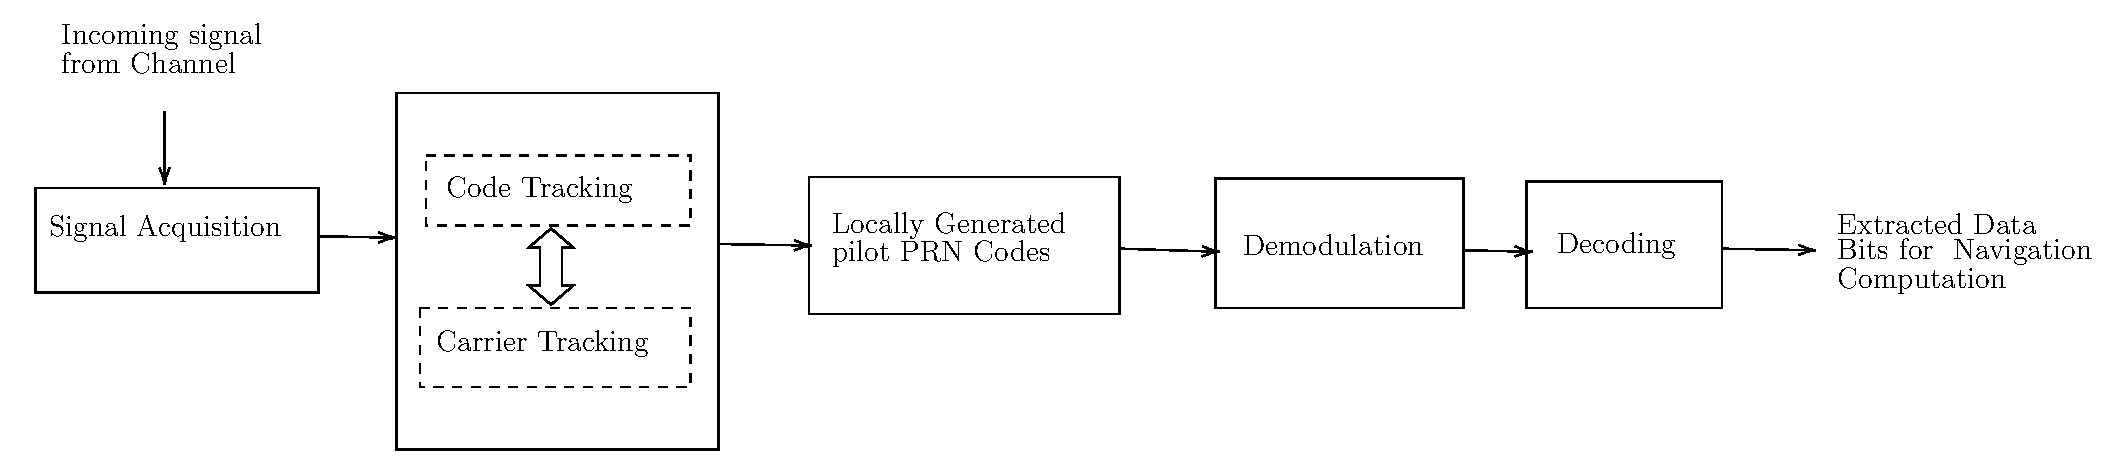
\includegraphics[width=1\columnwidth]{figs/signal_acq}
		\centering
		\captionsetup{justification=centering}
		\caption{The Block Level Architecture for Receiver}
		\label{fig:demod_flow}
	\end{figure}
\end{normalsize}
\\
\\
\begin{enumerate}
	\item \textbf{Signal acquisition:} The receiver searches for and acquires the NavIC signal for a given satellite(s) by correlating the received signal with a locally generated replica of the spreading code used by the satellite(s). This process helps in identifying the presence of the NavIC signal and estimating coarse value of both doppler frequency shift and code delay.
\item \textbf{Carrier tracking:} Once the signal is acquired, the receiver performs carrier tracking to estimate and track the carrier frequency and phase of the received signal. This is crucial for demodulation as it ensures accurate demodulation of the navigation message and ranging signal.
\item \textbf{Code delay tracking:} The receiver performs code delay tracking to estimate and track the spreading code used by the satellites. This helps in maintaining synchronization with the transmitted signal and extracting the navigation data and ranging information.
\item \textbf{Local Generation of pilot PRN:} The pilot PRN for every satellite is locally generated to determine the start of frame.
\item \textbf{Signal demodulation:}After the aquisition and tracking has been performed, the received data is mapped back using BPSK demodulation, mapping $-1$ to binary $1$ and $+1$ to binary $0$.
\item \textbf{Signal decoding:} Once the signal has been demodulated, the decoding is performed removing all the extra bits that were added to navigation data during the encoding process.
\end{enumerate}

\section{Signal Acquistion}
The role of the aqusition block is to examine the presence/absence of signals coming from a given satellite. In the case of signal being present, it should provide coarse estimations of the Code delay and the Carrier Doppler shift, yet accurate enough to initialize the frequency and code tracking loops.
\\
\\
A generic IRNSS signal defined by its complex baseband equivalent, 
$S_T(t)$, the digital signal at the input of an Acquisition block can be written as:
\begin{align}
	x_{IN}[k]=A(t)\hat s_T (t-\tau(t))e^{j(2 \pi f_D(t)t+\Phi(t))}\bigg|_{t=kT_s} +n(t)\bigg|_{t=kT_s}
\end{align}
\begin{table}[h]
%\centering
%%%%%%%%%%%%%%%%%%%%%%%%%%%%%%%%%%%%%%%%%%%%%%%%%%%%%%%%%%%%%%%%%%%%%%
%%                                                                  %%
%%  This is the header of a LaTeX2e file exported from Gnumeric.    %%
%%                                                                  %%
%%  This file can be compiled as it stands or included in another   %%
%%  LaTeX document. The table is based on the longtable package so  %%
%%  the longtable options (headers, footers...) can be set in the   %%
%%  preamble section below (see PRAMBLE).                           %%
%%                                                                  %%
%%  To include the file in another, the following two lines must be %%
%%  in the including file:                                          %%
%%        \def\inputGnumericTable{}                                 %%
%%  at the beginning of the file and:                               %%
%%        \input{name-of-this-file.tex}                             %%
%%  where the table is to be placed. Note also that the including   %%
%%  file must use the following packages for the table to be        %%
%%  rendered correctly:                                             %%
%%    \usepackage[latin1]{inputenc}                                 %%
%%    \usepackage{color}                                            %%
%%    \usepackage{array}                                            %%
%%    \usepackage{longtable}                                        %%
%%    \usepackage{calc}                                             %%
%%    \usepackage{multirow}                                         %%
%%    \usepackage{hhline}                                           %%
%%    \usepackage{ifthen}                                           %%
%%  optionally (for landscape tables embedded in another document): %%
%%    \usepackage{lscape}                                           %%
%%                                                                  %%
%%%%%%%%%%%%%%%%%%%%%%%%%%%%%%%%%%%%%%%%%%%%%%%%%%%%%%%%%%%%%%%%%%%%%%



%%  This section checks if we are begin input into another file or  %%
%%  the file will be compiled alone. First use a macro taken from   %%
%%  the TeXbook ex 7.7 (suggestion of Han-Wen Nienhuys).            %%
\def\ifundefined#1{\expandafter\ifx\csname#1\endcsname\relax}


%%  Check for the \def token for inputed files. If it is not        %%
%%  defined, the file will be processed as a standalone and the     %%
%%  preamble will be used.                                          %%
\ifundefined{inputGnumericTable}

%%  We must be able to close or not the document at the end.        %%
	\def\gnumericTableEnd{\end{document}}


%%%%%%%%%%%%%%%%%%%%%%%%%%%%%%%%%%%%%%%%%%%%%%%%%%%%%%%%%%%%%%%%%%%%%%
%%                                                                  %%
%%  This is the PREAMBLE. Change these values to get the right      %%
%%  paper size and other niceties.                                  %%
%%                                                                  %%
%%%%%%%%%%%%%%%%%%%%%%%%%%%%%%%%%%%%%%%%%%%%%%%%%%%%%%%%%%%%%%%%%%%%%%

	\documentclass[12pt%
			  %,landscape%
                    ]{report}
       \usepackage[latin1]{inputenc}
       \usepackage{fullpage}
       \usepackage{color}
       \usepackage{array}
       \usepackage{longtable}
       \usepackage{calc}
       \usepackage{multirow}
       \usepackage{hhline}
       \usepackage{ifthen}

	\begin{document}


%%  End of the preamble for the standalone. The next section is for %%
%%  documents which are included into other LaTeX2e files.          %%
\else

%%  We are not a stand alone document. For a regular table, we will %%
%%  have no preamble and only define the closing to mean nothing.   %%
    \def\gnumericTableEnd{}

%%  If we want landscape mode in an embedded document, comment out  %%
%%  the line above and uncomment the two below. The table will      %%
%%  begin on a new page and run in landscape mode.                  %%
%       \def\gnumericTableEnd{\end{landscape}}
%       \begin{landscape}


%%  End of the else clause for this file being \input.              %%
\fi

%%%%%%%%%%%%%%%%%%%%%%%%%%%%%%%%%%%%%%%%%%%%%%%%%%%%%%%%%%%%%%%%%%%%%%
%%                                                                  %%
%%  The rest is the gnumeric table, except for the closing          %%
%%  statement. Changes below will alter the table's appearance.     %%
%%                                                                  %%
%%%%%%%%%%%%%%%%%%%%%%%%%%%%%%%%%%%%%%%%%%%%%%%%%%%%%%%%%%%%%%%%%%%%%%

\providecommand{\gnumericmathit}[1]{#1} 
%%  Uncomment the next line if you would like your numbers to be in %%
%%  italics if they are italizised in the gnumeric table.           %%
%\renewcommand{\gnumericmathit}[1]{\mathit{#1}}
\providecommand{\gnumericPB}[1]%
{\let\gnumericTemp=\\#1\let\\=\gnumericTemp\hspace{0pt}}
 \ifundefined{gnumericTableWidthDefined}
        \newlength{\gnumericTableWidth}
        \newlength{\gnumericTableWidthComplete}
        \newlength{\gnumericMultiRowLength}
        \global\def\gnumericTableWidthDefined{}
 \fi
%% The following setting protects this code from babel shorthands.  %%
 \ifthenelse{\isundefined{\languageshorthands}}{}{\languageshorthands{english}}
%%  The default table format retains the relative column widths of  %%
%%  gnumeric. They can easily be changed to c, r or l. In that case %%
%%  you may want to comment out the next line and uncomment the one %%
%%  thereafter                                                      %%
\providecommand\gnumbox{\makebox[0pt]}
%%\providecommand\gnumbox[1][]{\makebox}

%% to adjust positions in multirow situations                       %%
\setlength{\bigstrutjot}{\jot}
\setlength{\extrarowheight}{\doublerulesep}

%%  The \setlongtables command keeps column widths the same across  %%
%%  pages. Simply comment out next line for varying column widths.  %%
\setlongtables

\setlength\gnumericTableWidth{%
	68pt+%
	235pt+%
0pt}
\def\gumericNumCols{2}
\setlength\gnumericTableWidthComplete{\gnumericTableWidth+%
         \tabcolsep*\gumericNumCols*2+\arrayrulewidth*\gumericNumCols}
\ifthenelse{\lengthtest{\gnumericTableWidthComplete > \linewidth}}%
         {\def\gnumericScale{\ratio{\linewidth-%
                        \tabcolsep*\gumericNumCols*2-%
                        \arrayrulewidth*\gumericNumCols}%
{\gnumericTableWidth}}}%
{\def\gnumericScale{1}}

%%%%%%%%%%%%%%%%%%%%%%%%%%%%%%%%%%%%%%%%%%%%%%%%%%%%%%%%%%%%%%%%%%%%%%
%%                                                                  %%
%% The following are the widths of the various columns. We are      %%
%% defining them here because then they are easier to change.       %%
%% Depending on the cell formats we may use them more than once.    %%
%%                                                                  %%
%%%%%%%%%%%%%%%%%%%%%%%%%%%%%%%%%%%%%%%%%%%%%%%%%%%%%%%%%%%%%%%%%%%%%%

\ifthenelse{\isundefined{\gnumericColA}}{\newlength{\gnumericColA}}{}\settowidth{\gnumericColA}{\begin{tabular}{@{}p{68pt*\gnumericScale}@{}}x\end{tabular}}
\ifthenelse{\isundefined{\gnumericColB}}{\newlength{\gnumericColB}}{}\settowidth{\gnumericColB}{\begin{tabular}{@{}p{235pt*\gnumericScale}@{}}x\end{tabular}}

\begin{longtable}[c]{%
	b{\gnumericColA}%
	b{\gnumericColB}%
	}

%%%%%%%%%%%%%%%%%%%%%%%%%%%%%%%%%%%%%%%%%%%%%%%%%%%%%%%%%%%%%%%%%%%%%%
%%  The longtable options. (Caption, headers... see Goosens, p.124) %%
%	\caption{The Table Caption.}             \\	%
% \hline	% Across the top of the table.
%%  The rest of these options are table rows which are placed on    %%
%%  the first, last or every page. Use \multicolumn if you want.    %%

%%  Header for the first page.                                      %%
%	\multicolumn{2}{c}{The First Header} \\ \hline 
%	\multicolumn{1}{c}{colTag}	%Column 1
%	&\multicolumn{1}{c}{colTag}	\\ \hline %Last column
%	\endfirsthead

%%  The running header definition.                                  %%
%	\hline
%	\multicolumn{2}{l}{\ldots\small\slshape continued} \\ \hline
%	\multicolumn{1}{c}{colTag}	%Column 1
%	&\multicolumn{1}{c}{colTag}	\\ \hline %Last column
%	\endhead

%%  The running footer definition.                                  %%
%	\hline
%	\multicolumn{2}{r}{\small\slshape continued\ldots} \\
%	\endfoot

%%  The ending footer definition.                                   %%
%	\multicolumn{2}{c}{That's all folks} \\ \hline 
%	\endlastfoot
%%%%%%%%%%%%%%%%%%%%%%%%%%%%%%%%%%%%%%%%%%%%%%%%%%%%%%%%%%%%%%%%%%%%%%

\hhline{|-|-}
	 \multicolumn{1}{|p{\gnumericColA}|}%
	{\gnumericPB{\raggedright}\gnumbox[l]{\hspace{0.75cm}\textbf{Symbol}}}
	&\multicolumn{1}{p{\gnumericColB}|}%
	{\gnumericPB{\raggedright}\gnumbox[l]{\hspace{3cm} \textbf{Definition}}}
\\
\hhline{|--|}
	 \multicolumn{1}{|p{\gnumericColA}|}%
	{\gnumericPB{\raggedright}\gnumbox[l]{\hspace{1cm}$x_{IN}[k]$}}
	&\multicolumn{1}{p{\gnumericColB}|}%
	{\gnumericPB{\raggedright}\gnumbox[l]{Complex vector $I,Q$ samples of received signal}}
\\
\hhline{|--|}
	 \multicolumn{1}{|p{\gnumericColA}|}%
	{\gnumericPB{\raggedright}\gnumbox[l]{\hspace{1cm}A(t)}}
	&\multicolumn{1}{p{\gnumericColB}|}%
	{\gnumericPB{\raggedright}\gnumbox[l]{Signal Amplitude}}
\\
\hhline{|--|}
	 \multicolumn{1}{|p{\gnumericColA}|}%
	{\gnumericPB{\raggedright}\gnumbox[l]{\hspace{1cm}$\hat s_T(t)$}}
	&\multicolumn{1}{p{\gnumericColB}|}%
	{\gnumericPB{\raggedright}\gnumbox[l]{filtered version of $s_T(t)$}}
\\
\hhline{|--|}
	 \multicolumn{1}{|p{\gnumericColA}|}%
	{\gnumericPB{\raggedright}\gnumbox[l]{\hspace{1cm}$f_D(t)$ }}
	&\multicolumn{1}{p{\gnumericColB}|}%
	{\gnumericPB{\raggedright}\gnumbox[l]{Time varying doppler shift}}
\\
\hhline{|--|}
	 \multicolumn{1}{|p{\gnumericColA}|}%
	{\gnumericPB{\raggedright}\gnumbox[l]{\hspace{1cm}$\Phi (t)$}}
	&\multicolumn{1}{p{\gnumericColB}|}%
	{\gnumericPB{\raggedright}\gnumbox[l]{Time varying carrier phase shift}}
\\
\hhline{|--|}
	 \multicolumn{1}{|p{\gnumericColA}|}%
	{\gnumericPB{\raggedright}\gnumbox[l]{\hspace{1cm}$\tau (t)$}}
	&\multicolumn{1}{p{\gnumericColB}|}%
	{\gnumericPB{\raggedright}\gnumbox[l]{Time varying code delay}}
\\
\hhline{|--|}
	 \multicolumn{1}{|p{\gnumericColA}|}%
	{\gnumericPB{\raggedright}\gnumbox[l]{\hspace{1cm}n(t) }}
	&\multicolumn{1}{p{\gnumericColB}|}%
	{\gnumericPB{\raggedright}\gnumbox[l]{Time varying random noise}}
\\
\hhline{|--|}
	 \multicolumn{1}{|p{\gnumericColA}|}%
	{\gnumericPB{\raggedright}\gnumbox[l]{\hspace{1cm}$T_s$ }}
	&\multicolumn{1}{p{\gnumericColB}|}%
	{\gnumericPB{\raggedright}\gnumbox[l]{Sampling period}}
\\
\hhline{|-|-|}
\end{longtable}

\ifthenelse{\isundefined{\languageshorthands}}{}{\languageshorthands{\languagename}}
\gnumericTableEnd

\vspace{3mm}
\caption{Parameters Table in Signal Acquisition}
\label{table:table_para}
\end{table}

\subsection{Implementation of CA PCPS Acquisition}
The Parallel Code Phase Search (PCPS) algorithm is used in Acquisition block and is depicted in figure \ref{fig:pcps_flow} and described as follows:
\begin{normalsize}
\begin{figure}[ht]
	\centering
	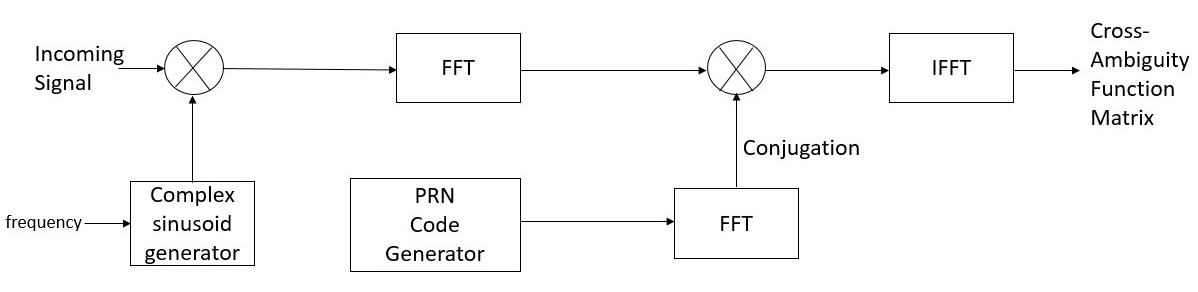
\includegraphics[width=1\columnwidth]{figs/pcps}
	\centering
	\captionsetup{justification=centering}
	\caption{PCPS algorithm flow}
	\label{fig:pcps_flow}
\end{figure}
\end{normalsize}
\\
\textbf{Given:}
\begin{enumerate}
	\item Input signal buffer $x_{IN}$ of K complex samples, provided by the Signal Conditioner 
	\item On-memory FFT of the local replica
	\begin{align}
		D[k]=FFT_K\{d[k]\}
	\end{align}
	\item Acquisition threshold  $\gamma$
	\item Frequency span : \sbrak{f_{min}, f_{max}}
	\item Frequency step : $f_{step}$
\end{enumerate}
\textbf{Expected:}
\begin{enumerate}
	\item Find out if signal is acquired or not for a given satellite(s) 
	\item If signal is acquired, for each given satellite, calculate coarse estimation of Doppler shift $\hat f_{D_{acq}}$ and Code delay $\hat \tau_{acq}$
\end{enumerate}
\textbf{Algorithm:}
\begin{enumerate}
	\item Calculate input signal power estimation  $\hat P_{in} = \frac{1}{K}\sum_{k=0}^{K-1} \big| x_{IN}[k]\big| ^2$
	\item for $\check f_D=[ f_{min} to f_{max}]\text{ in }f_{steps}$ 
	\begin{enumerate}
		\item Calculate carrier wipe off$\hspace{0.5cm}x[k]=x_{IN}[k]e^{-(j2 \pi \check f_D k T_s)}$,for $k=0,...,K-1$
		\item Calculate $X[k]=FFT_K\{x[k]\}$
		\item Calculate $Y[k]=X[k].D[k]$, for $k=0,...K-1$ 
        	\item Calculate corresponding column in the Cross ambiguity function matrix - $R_{xd}(\check f_D,\tau) = \frac{1}{K^2}IFFT_K\{Y[k]\}$
        \end{enumerate}

        \item Search maximum and its indices in the search grid:
	\begin{align}
		\{S_{max},f_i,\tau_j\} = max_{f,\tau} \big |R_{xd}(f,\tau)\big | ^2
	\end{align}
        \item	Calculate the Generalized Likelihood Ratio Test (GLRT) function with normalized variance:
	\begin{align}
		\Gamma_{GLRT} = \frac{2KS_{max}}{\hat P_{in}}
	\end{align}
	\item if $\Gamma_{GLRT} > \gamma$\\
	Declare positive acquisition and provides coarse estimation of code delay $\hat \tau_{acq} = \tau_j $ and Doppler shift $\hat f_{D_{acq}}=f_i$,\\
	other wise declare negative acquisition.\\
\end{enumerate}


\section{Tracking}
The role of tracking block is to follow signal synchronization parameters: code phase, Doppler shift and carrier phase and extract the baseband signal. It performs the following 3 function to decipher the baseband signal from the incoming signal as shown in figure \ref{fig:tracking}. 
\begin{enumerate}
	\item Carrier and code wipeoff 
	\item Pre-detection integration
	\item Baseband signal processing
\end{enumerate}

\begin{normalsize}
\begin{figure}[ht]
\centering
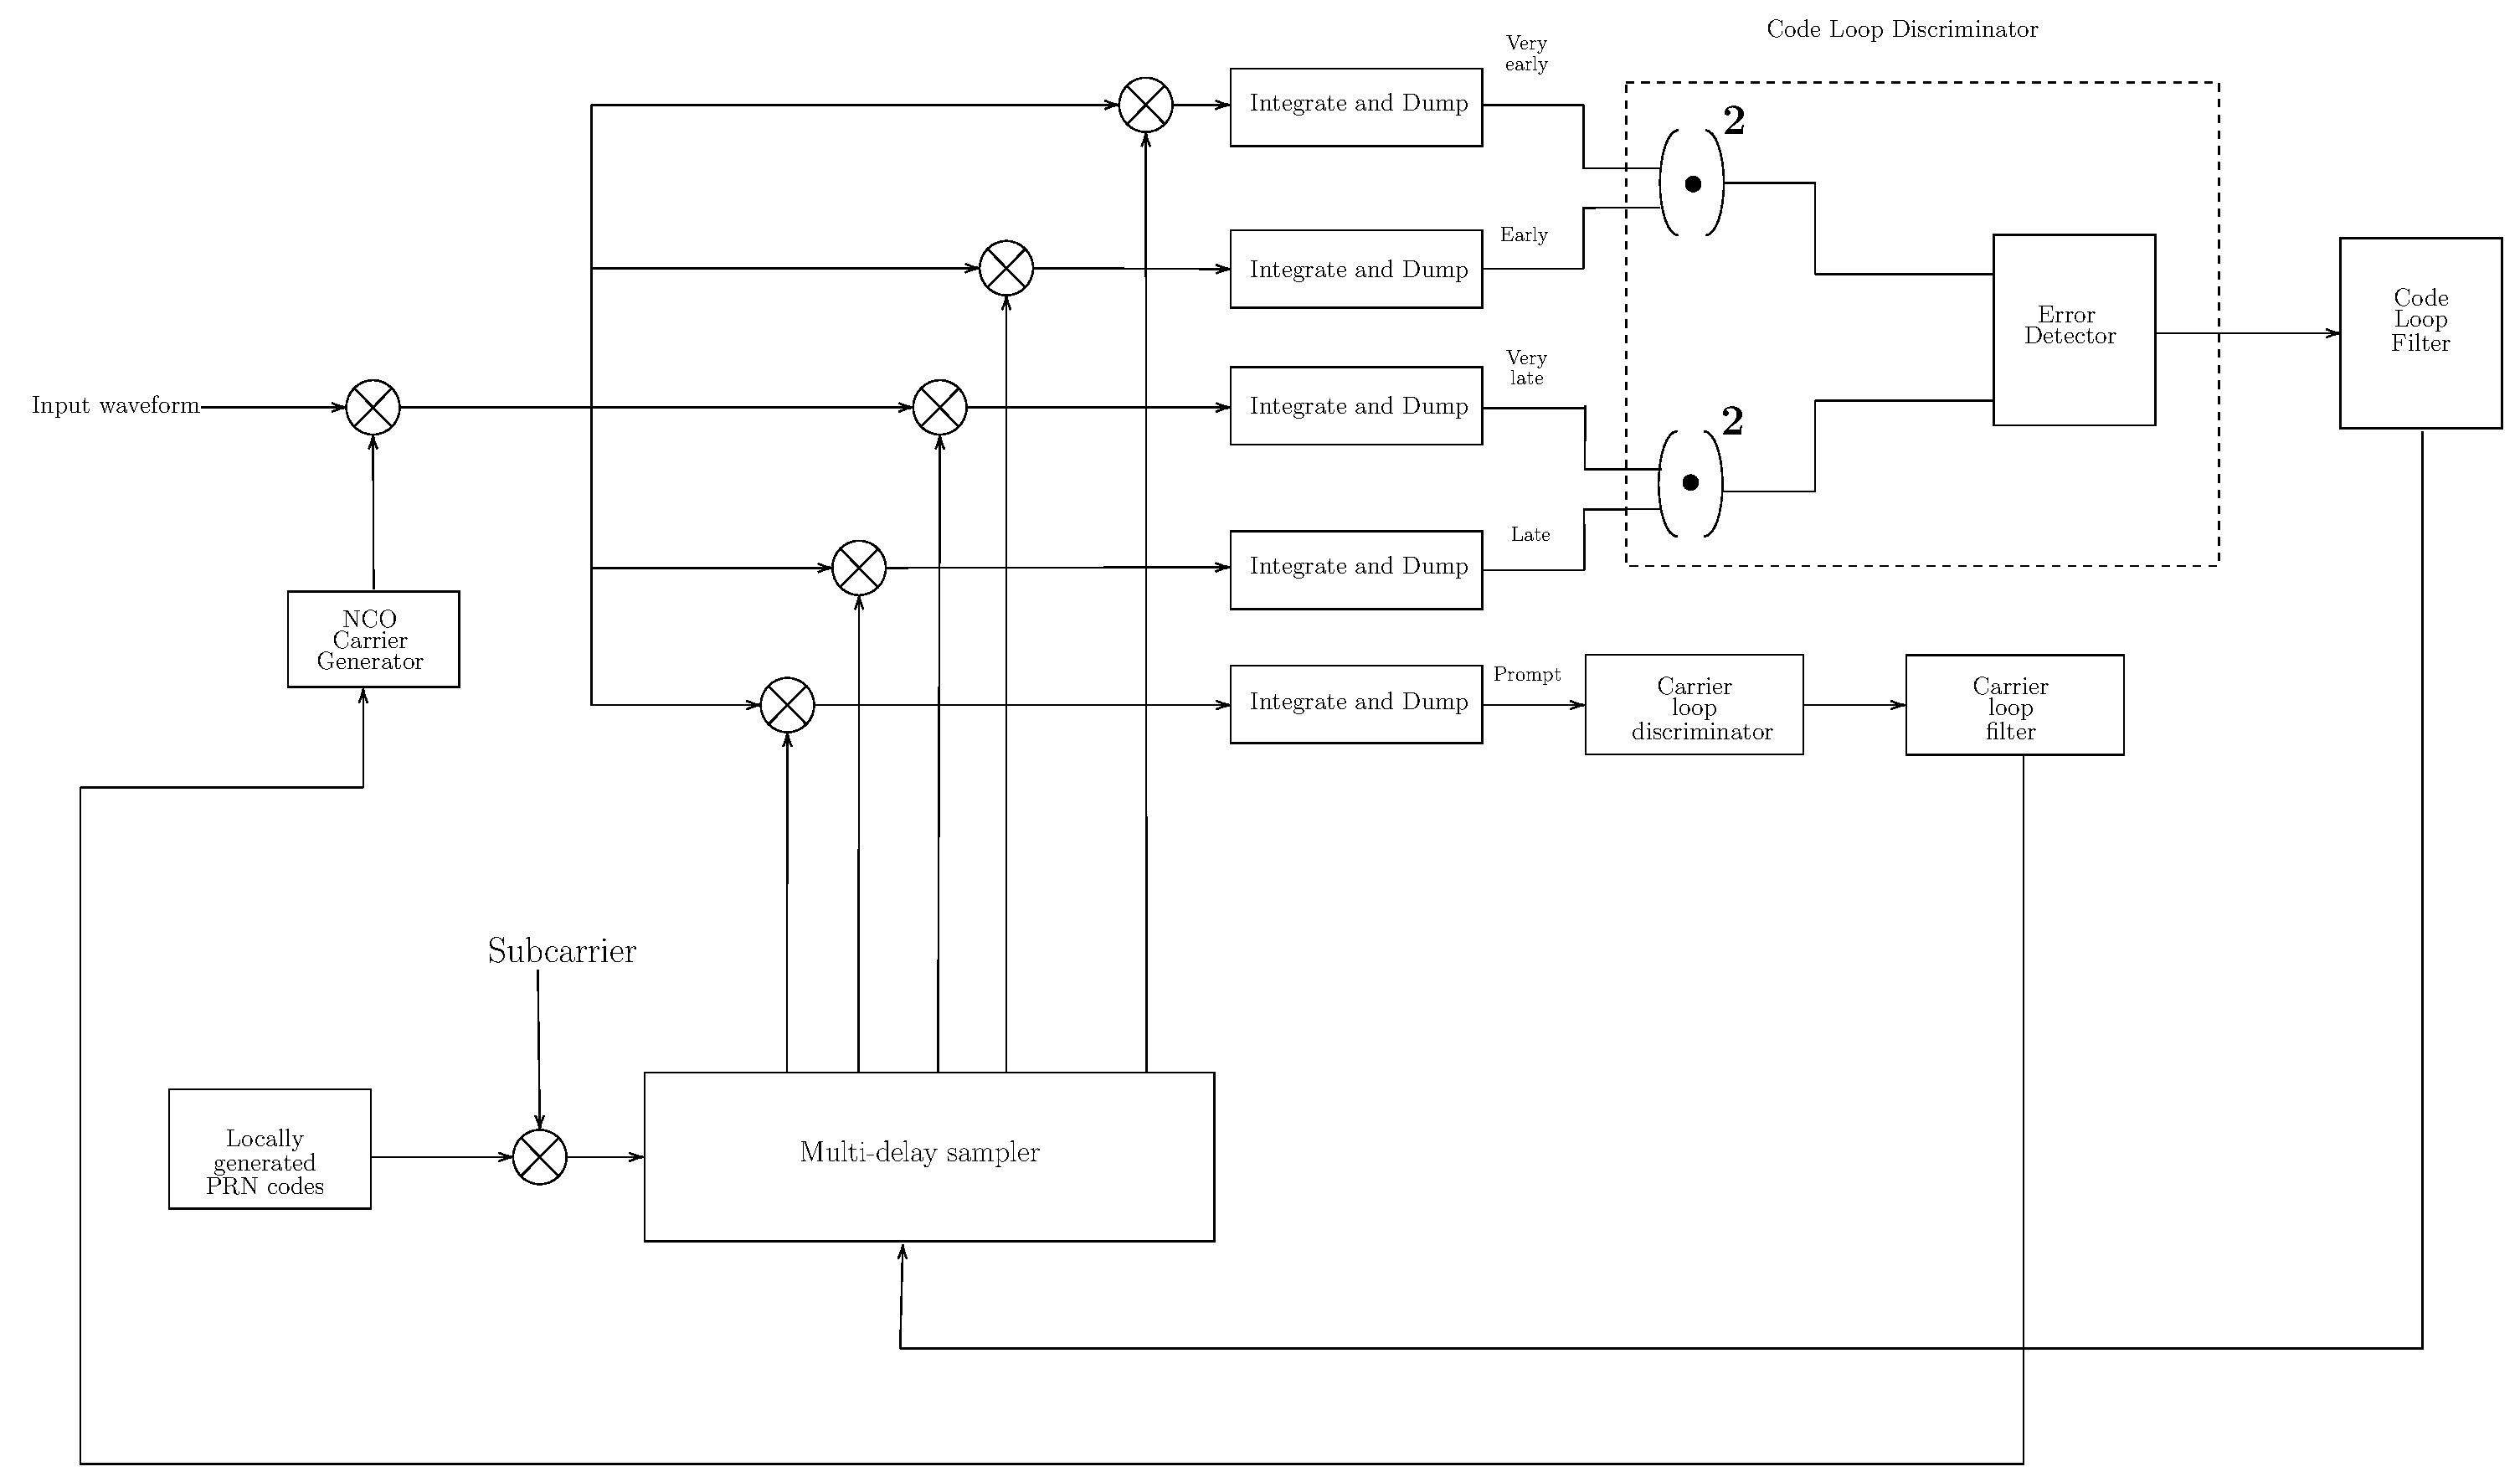
\includegraphics[width=1.25\columnwidth]{figs/tracking}
\centering
\captionsetup{justification=centering}
\caption{Tracking block diagram}
\label{fig:tracking}
\end{figure}
\end{normalsize}
\subsection{Carrier and code wipeoff}
\textbf{Carrier wipeoff: }Referring to the figure \ref{fig:tracking}, first the incoming signal is stripped off the carrier (plus carrier Doppler) by the replica carrier (plus carrier Doppler) signals. The replica carrier (including carrier Doppler) signals are synthesized by the carrier numerically controlled oscillator (NCO). In closed loop operation, the carrier NCO is controlled by the carrier tracking loop in the receiver processor.
\\
\textbf{Code wipeoff: } The received signal is then correlated with very early(VE), early(E), prompt(P), late(L) and very late(VL) replica codes (plus code Doppler) synthesized by a multi-delay sampler. In the closed loop operation, the code NCO is controlled by the code tracking loop in the receiver processor. E and L are typically separated in phase by 0.3 chips and P is in the middle. VE and VL are separated by 1.2 chips. The prompt replica code phase is aligned with the incoming satellite code phase producing maximum correlation if it is tracking the incoming satellite code phase. Under this circumstance, the early phase is aligned a fraction of a chip period early, and the late phase is aligned the same fraction of the chip period late with respect to the incoming  code phase, and these correlators produce about half the maximum correlation. Any misalignment in the replica code phase with respect to the incoming code phase produces a difference in the vector magnitudes of the early and late correlated outputs so that the amount and direction of the phase change can be detected and corrected by the code tracking loop.
\subsection{Pre-detection and integration}
Extensive digital predetection integration and dump processes occur after the carrier and code wiping off processes. Figure \ref{fig:tracking} shows five complex correlators required to produce five
components, which are integrated and dumped to produce very early, early, prompt, late and very late vesions of the signal . The carrier wipeoff and code wipeoff processes must be performed at the digital IF sample rate, while the integrate and dump accumulators provide filtering and resampling at the processor baseband input rate, which can be at 1,000 Hz during search modes or as low as 50 Hz during
track modes, depending on the desired dwell time during search or the desired predetection integration time during track.
\subsection{Baseband signal processing}
This entails Carrier tracking and Code tracking using Phase locked loop (PLL), Frequency locked loop (FLL) and Delay locked loop (DLL). 


\subsubsection{Carrier tracking loop}
\textbf{Phase locked loop(PLL)}\\
The carrier loop discriminator defines the type of tracking loop as a PLL, a Costas PLL (which is a PLL-type discriminator that tolerates the presence of data modulation on the baseband signal), or a frequency lock loop (FLL). Carrier tracking loop tracks the frequency and phase of the received signal by detecting the phase error between replicated signal and incoming signal and accordingly replicated signal produced by numerically controlled oscillator (NCO) is adjusted to synchronize with incoming signal in both frequency and phase. For zero phase error detected, navigation data is accurately extracted. 
\begin{align}
  %\text{Phase error} =ATAN2(I_P,Q_P) = \tan^{-1}\brak{\frac{I_P}{Q_P}}
  \text{Phase error}_{pilot} &=ATAN2(I_P,Q_P) = \tan^{-1}\brak{\frac{I_P}{Q_P}}\\
  \text{Phase error}_{data} &=ATAN2(Q_P,I_P) = \tan^{-1}\brak{\frac{Q_P}{I_P}}
\end{align}
The ATAN2 discriminator is the only one that remains linear over the full input error range of $\pm180^{\circ}$. However, in the presence of noise, both of the discriminator outputs are linear only near the $0^{\circ}$ region. These PLL discriminators will achieve the 6-dB improvement in signal tracking threshold (by comparison with the Costas discriminators) for the dataless carrier because they track the full four quadrant range of the input signal.
\\
\\
\textbf{Frequency locked loop}\\
PLLs replicate the exact phase and frequency of the incoming SV (converted to IF) to perform the carrier wipeoff function. FLLs perform the carrier wipeoff process by replicating the approximate frequency, and they typically permit the phase to rotate with respect to the incoming carrier signal. The algorithm used in FLL discriminator is $\frac{\text{ATAN2}{\brak{cross,dot}}}{t_2-t_1}$. The frequency error is given by 
\begin{align}
	\text{Frequency error} = \frac{\phi_2-\phi_1}{t_2-t_1}
\end{align}

\noindent The phase change $\phi_2 - \phi_1$ between two adjacent samples of $I_{PS}$ and $Q_{PS}$ at times $t_2$ and $t_1$ is computed. This phase change in a fixed interval of time is proportinal to frequenct error in the carrier tracking loop. The error is fed to carier NCO to adjust the frequency to lock to the right frequency.

\subsubsection{Code tracking loop}
\textbf{Delay locked loop:}
Post the carrier signal synchronization, received CA code samples are synchronized by aligning with replicated CA code samples by shifting right or left. To determine the direction of shift, the I and Q outputs are multiplied with prompt code (PRN code which is phase aligned), early code (prompt PRN code shifted by some samples to the right) and late code (prompt PRN code shifted by some samples to the left) resulting in corresponding to I and Q channel respectively. Following algorithm is used to lock the code phase.

\begin{align}
	E_K&=\sqrt[]{VE^2+E^2}\\
	L_K&=\sqrt[]{VL^2+L^2}
\end{align}

\begin{align}
	\text{DLL Discriminator} (\epsilon)&=\frac{1}{2}\frac{E_K-L_K}{E_K+L_K}
\end{align}

\noindent If the replica code is aligned, then the early and late envelopes are equal in amplitude and no error is generated by the discriminator. If the replica code is misaligned, then the early and late envelopes are unequal by an amount that is proportional to the amount of code phase error between the replica and the incoming signal (within the limits of the correlation interval). The code discriminator senses the amount of error in the replica code and the direction (early or late) from the difference in the amplitudes of the early and late envelopes. This
error is filtered and then applied to the code loop NCO, where the output code shift is increased or decreased as necessary to correct the replica code generator phase with respect to the incoming SV signal code phase.

\subsubsection{Loop filter characteristics}
\begin{table}[h]
%\centering
%%%%%%%%%%%%%%%%%%%%%%%%%%%%%%%%%%%%%%%%%%%%%%%%%%%%%%%%%%%%%%%%%%%%%%
%%                                                                  %%
%%  This is the header of a LaTeX2e file exported from Gnumeric.    %%
%%                                                                  %%
%%  This file can be compiled as it stands or included in another   %%
%%  LaTeX document. The table is based on the longtable package so  %%
%%  the longtable options (headers, footers...) can be set in the   %%
%%  preamble section below (see PRAMBLE).                           %%
%%                                                                  %%
%%  To include the file in another, the following two lines must be %%
%%  in the including file:                                          %%
%%        \def\inputGnumericTable{}                                 %%
%%  at the beginning of the file and:                               %%
%%        \input{name-of-this-file.tex}                             %%
%%  where the table is to be placed. Note also that the including   %%
%%  file must use the following packages for the table to be        %%
%%  rendered correctly:                                             %%
%%    \usepackage[latin1]{inputenc}                                 %%
%%    \usepackage{color}                                            %%
%%    \usepackage{array}                                            %%
%%    \usepackage{longtable}                                        %%
%%    \usepackage{calc}                                             %%
%%    \usepackage{multirow}                                         %%
%%    \usepackage{hhline}                                           %%
%%    \usepackage{ifthen}                                           %%
%%  optionally (for landscape tables embedded in another document): %%
%%    \usepackage{lscape}                                           %%
%%                                                                  %%
%%%%%%%%%%%%%%%%%%%%%%%%%%%%%%%%%%%%%%%%%%%%%%%%%%%%%%%%%%%%%%%%%%%%%%



%%  This section checks if we are begin input into another file or  %%
%%  the file will be compiled alone. First use a macro taken from   %%
%%  the TeXbook ex 7.7 (suggestion of Han-Wen Nienhuys).            %%
\def\ifundefined#1{\expandafter\ifx\csname#1\endcsname\relax}


%%  Check for the \def token for inputed files. If it is not        %%
%%  defined, the file will be processed as a standalone and the     %%
%%  preamble will be used.                                          %%
\ifundefined{inputGnumericTable}

%%  We must be able to close or not the document at the end.        %%
	\def\gnumericTableEnd{\end{document}}


%%%%%%%%%%%%%%%%%%%%%%%%%%%%%%%%%%%%%%%%%%%%%%%%%%%%%%%%%%%%%%%%%%%%%%
%%                                                                  %%
%%  This is the PREAMBLE. Change these values to get the right      %%
%%  paper size and other niceties.                                  %%
%%                                                                  %%
%%%%%%%%%%%%%%%%%%%%%%%%%%%%%%%%%%%%%%%%%%%%%%%%%%%%%%%%%%%%%%%%%%%%%%

	\documentclass[12pt%
			  %,landscape%
                    ]{report}
       \usepackage[latin1]{inputenc}
       \usepackage{fullpage}
       \usepackage{color}
       \usepackage{array}
       \usepackage{longtable}
       \usepackage{calc}
       \usepackage{multirow}
       \usepackage{hhline}
       \usepackage{ifthen}

	\begin{document}


%%  End of the preamble for the standalone. The next section is for %%
%%  documents which are included into other LaTeX2e files.          %%
\else

%%  We are not a stand alone document. For a regular table, we will %%
%%  have no preamble and only define the closing to mean nothing.   %%
    \def\gnumericTableEnd{}

%%  If we want landscape mode in an embedded document, comment out  %%
%%  the line above and uncomment the two below. The table will      %%
%%  begin on a new page and run in landscape mode.                  %%
%       \def\gnumericTableEnd{\end{landscape}}
%       \begin{landscape}


%%  End of the else clause for this file being \input.              %%
\fi

%%%%%%%%%%%%%%%%%%%%%%%%%%%%%%%%%%%%%%%%%%%%%%%%%%%%%%%%%%%%%%%%%%%%%%
%%                                                                  %%
%%  The rest is the gnumeric table, except for the closing          %%
%%  statement. Changes below will alter the table's appearance.     %%
%%                                                                  %%
%%%%%%%%%%%%%%%%%%%%%%%%%%%%%%%%%%%%%%%%%%%%%%%%%%%%%%%%%%%%%%%%%%%%%%

\providecommand{\gnumericmathit}[1]{#1} 
%%  Uncomment the next line if you would like your numbers to be in %%
%%  italics if they are italizised in the gnumeric table.           %%
%\renewcommand{\gnumericmathit}[1]{\mathit{#1}}
\providecommand{\gnumericPB}[1]%
{\let\gnumericTemp=\\#1\let\\=\gnumericTemp\hspace{0pt}}
 \ifundefined{gnumericTableWidthDefined}
        \newlength{\gnumericTableWidth}
        \newlength{\gnumericTableWidthComplete}
        \newlength{\gnumericMultiRowLength}
        \global\def\gnumericTableWidthDefined{}
 \fi
%% The following setting protects this code from babel shorthands.  %%
 \ifthenelse{\isundefined{\languageshorthands}}{}{\languageshorthands{english}}
%%  The default table format retains the relative column widths of  %%
%%  gnumeric. They can easily be changed to c, r or l. In that case %%
%%  you may want to comment out the next line and uncomment the one %%
%%  thereafter                                                      %%
\providecommand\gnumbox{\makebox[0pt]}
%%\providecommand\gnumbox[1][]{\makebox}

%% to adjust positions in multirow situations                       %%
\setlength{\bigstrutjot}{\jot}
\setlength{\extrarowheight}{\doublerulesep}

%%  The \setlongtables command keeps column widths the same across  %%
%%  pages. Simply comment out next line for varying column widths.  %%
\setlongtables

\setlength\gnumericTableWidth{%
	70pt+%
	100pt+%
	80pt+%
0pt}
\def\gumericNumCols{3}
\setlength\gnumericTableWidthComplete{\gnumericTableWidth+%
         \tabcolsep*\gumericNumCols*2+\arrayrulewidth*\gumericNumCols}
\ifthenelse{\lengthtest{\gnumericTableWidthComplete > \linewidth}}%
         {\def\gnumericScale{\ratio{\linewidth-%
                        \tabcolsep*\gumericNumCols*2-%
                        \arrayrulewidth*\gumericNumCols}%
{\gnumericTableWidth}}}%
{\def\gnumericScale{1}}

%%%%%%%%%%%%%%%%%%%%%%%%%%%%%%%%%%%%%%%%%%%%%%%%%%%%%%%%%%%%%%%%%%%%%%
%%                                                                  %%
%% The following are the widths of the various columns. We are      %%
%% defining them here because then they are easier to change.       %%
%% Depending on the cell formats we may use them more than once.    %%
%%                                                                  %%
%%%%%%%%%%%%%%%%%%%%%%%%%%%%%%%%%%%%%%%%%%%%%%%%%%%%%%%%%%%%%%%%%%%%%%

\ifthenelse{\isundefined{\gnumericColA}}{\newlength{\gnumericColA}}{}\settowidth{\gnumericColA}{\begin{tabular}{@{}p{70pt*\gnumericScale}@{}}x\end{tabular}}
\ifthenelse{\isundefined{\gnumericColB}}{\newlength{\gnumericColB}}{}\settowidth{\gnumericColB}{\begin{tabular}{@{}p{100pt*\gnumericScale}@{}}x\end{tabular}}
\ifthenelse{\isundefined{\gnumericColC}}{\newlength{\gnumericColC}}{}\settowidth{\gnumericColC}{\begin{tabular}{@{}p{80pt*\gnumericScale}@{}}x\end{tabular}}

\begin{longtable}[c]{%
	b{\gnumericColA}%
	b{\gnumericColB}%
	b{\gnumericColC}%
	}

%%%%%%%%%%%%%%%%%%%%%%%%%%%%%%%%%%%%%%%%%%%%%%%%%%%%%%%%%%%%%%%%%%%%%%
%%  The longtable options. (Caption, headers... see Goosens, p.124) %%
%	\caption{The Table Caption.}             \\	%
% \hline	% Across the top of the table.
%%  The rest of these options are table rows which are placed on    %%
%%  the first, last or every page. Use \multicolumn if you want.    %%

%%  Header for the first page.                                      %%
%	\multicolumn{3}{c}{The First Header} \\ \hline 
%	\multicolumn{1}{c}{colTag}	%Column 1
%	&\multicolumn{1}{c}{colTag}	%Column 2
%	&\multicolumn{1}{c}{colTag}	\\ \hline %Last column
%	\endfirsthead

%%  The running header definition.                                  %%
%	\hline
%	\multicolumn{3}{l}{\ldots\small\slshape continued} \\ \hline
%	\multicolumn{1}{c}{colTag}	%Column 1
%	&\multicolumn{1}{c}{colTag}	%Column 2
%	&\multicolumn{1}{c}{colTag}	\\ \hline %Last column
%	\endhead

%%  The running footer definition.                                  %%
%	\hline
%	\multicolumn{3}{r}{\small\slshape continued\ldots} \\
%	\endfoot

%%  The ending footer definition.                                   %%
%	\multicolumn{3}{c}{That's all folks} \\ \hline 
%	\endlastfoot
%%%%%%%%%%%%%%%%%%%%%%%%%%%%%%%%%%%%%%%%%%%%%%%%%%%%%%%%%%%%%%%%%%%%%%

\hhline{|-|-|-}
	 \multicolumn{1}{|p{\gnumericColA}|}%
	{\gnumericPB{\raggedright}\gnumbox[l]{\textbf{Loop Order}}}
	&\multicolumn{1}{p{\gnumericColB}|}%
	{\gnumericPB{\raggedright}\gnumbox[l]{\textbf{Noise Bandwidth}}}
	&\multicolumn{1}{p{\gnumericColC}|}%
	{\gnumericPB{\raggedright}\gnumbox[l]{\textbf{Typical Filter  }}}
\\
%\hhline{|---|}
	 \multicolumn{1}{|p{\gnumericColA}|}%
	{\gnumericPB{\raggedleft}\gnumbox[r]{}}
	&\multicolumn{1}{p{\gnumericColB}|}%
	{\gnumericPB{\raggedright}\gnumbox[l]{\textbf{$ B_n$ (Hz)}}}
	&\multicolumn{1}{p{\gnumericColC}|}%
	{\gnumericPB{\raggedright}\gnumbox[l]{\textbf{ Values }}}
	%{\gnumericPB{\raggedright}\gnumbox[l]{}}\\
	\\
\hhline{|---|}
	 \multicolumn{1}{|p{\gnumericColA}|}%
	{\gnumericPB{\raggedleft}\gnumbox[r]{First}}
	&\multicolumn{1}{p{\gnumericColB}|}%
	{\gnumericPB{\raggedright}\gnumbox[l]{\hspace{0.5cm}$\frac{\omega_o}{4}$}}
	&\multicolumn{1}{p{\gnumericColC}|}%
	{\gnumericPB{\raggedright}\gnumbox[l]{\hspace{0.5cm}$\omega_o $ }}
	%{\gnumericPB{\raggedright}\gnumbox[l]{}}\\
	\\
%\hhline{|---|}
	 \multicolumn{1}{|p{\gnumericColA}|}%
	{\gnumericPB{\raggedleft}\gnumbox[r]{}}
	&\multicolumn{1}{p{\gnumericColB}|}%
	{\gnumericPB{\raggedright}\gnumbox[l]{}}
	&\multicolumn{1}{p{\gnumericColC}|}%
	{\gnumericPB{\raggedright}\gnumbox[l]{ $B_n=0.25\omega_o$}}
\\
\hhline{|---|}
\multicolumn{1}{|p{\gnumericColA}|}%
	{\gnumericPB{\raggedleft}\gnumbox[r]{}}
	&\multicolumn{1}{p{\gnumericColB}|}%
	{\gnumericPB{\raggedright}\gnumbox[l]{}}
	&\multicolumn{1}{p{\gnumericColC}|}%
	{\gnumericPB{\raggedright}\gnumbox[l]{ $\omega_o^2$}}
	 
\\
%\hhline{|---|}
	\multicolumn{1}{|p{\gnumericColA}|}%
	{\gnumericPB{\raggedleft}\gnumbox[r]{Second}}
	&\multicolumn{1}{p{\gnumericColB}|}%
	{\gnumericPB{\raggedright}\gnumbox[l]{$\frac{\omega(1+a_2^2)}{4a_2}$}}
	&\multicolumn{1}{p{\gnumericColC}|}%
	{\gnumericPB{\raggedright}\gnumbox[l]{$a_2\omega_o=1.414\omega_o$}}
\\
%\hhline{|-|-|-|}
\multicolumn{1}{|p{\gnumericColA}|}%
	{\gnumericPB{\raggedleft}\gnumbox[r]{}}
	&\multicolumn{1}{p{\gnumericColB}|}%
	{\gnumericPB{\raggedright}\gnumbox[l]{}}
	&\multicolumn{1}{p{\gnumericColC}|}%
	{\gnumericPB{\raggedright}\gnumbox[l]{ $B_n=0.53\omega_o$}}
	
	\\
\hhline{|-|-|-|}
 \multicolumn{1}{|p{\gnumericColA}|}%
	{\gnumericPB{\raggedleft}\gnumbox[r]{}}
	&\multicolumn{1}{p{\gnumericColB}|}%
	{\gnumericPB{\raggedright}\gnumbox[l]{}}
	&\multicolumn{1}{p{\gnumericColC}|}%
	{\gnumericPB{\raggedright}\gnumbox[l]{$\omega_o^3$ }}
		\\
%\hhline{|-|-|-|}
 \multicolumn{1}{|p{\gnumericColA}|}%
	{\gnumericPB{\raggedleft}\gnumbox[r]{Third}}
	&\multicolumn{1}{p{\gnumericColB}|}%
	{\gnumericPB{\raggedright}\gnumbox[l]{$\frac{\omega(a_3b_3^2+a_3^2-b_3)}{4(a_3b_3-1)}$}}
	&\multicolumn{1}{p{\gnumericColC}|}%
	{\gnumericPB{\raggedright}\gnumbox[l]{$ a_3\omega_o^2=1.1\omega_o^2$}}
	\\
%\hhline{|-|-|-|}
 \multicolumn{1}{|p{\gnumericColA}|}%
	{\gnumericPB{\raggedleft}\gnumbox[r]{}}
	&\multicolumn{1}{p{\gnumericColB}|}%
	{\gnumericPB{\raggedright}\gnumbox[l]{}}
	&\multicolumn{1}{p{\gnumericColC}|}%
	{\gnumericPB{\raggedright}\gnumbox[l]{$b_3\omega_o=2.4\omega_o$}}
	\\
%\hhline{|-|-|-|}
 \multicolumn{1}{|p{\gnumericColA}|}%
	{\gnumericPB{\raggedleft}\gnumbox[r]{}}
	&\multicolumn{1}{p{\gnumericColB}|}%
	{\gnumericPB{\raggedright}\gnumbox[l]{}}
	&\multicolumn{1}{p{\gnumericColC}|}%
	{\gnumericPB{\raggedright}\gnumbox[l]{ $B_n=0.7845\omega_o$}}
		\\
\hhline{|-|-|-|}
 
\end{longtable}

\ifthenelse{\isundefined{\languageshorthands}}{}{\languageshorthands{\languagename}}
\gnumericTableEnd

\vspace{3mm}
\caption{Loop order filters}
\label{table:loop}
\end{table}
\noindent The values for the second-order coefficient $a_2$ and third-order coefficients $a_3$ and $b_3$ can be determined from Table 3. These coefficients are the same for FLL, PLL, or DLL applications if the loop
order and the noise bandwidth,$B_n$ , are the same.Note that the FLL coefficient insertion point into the filter is one integrator back from the PLL and DLL insertion points.This is because the FLL error is in units of hertz (change in range per unit of time).

\section{Local PRN Generation}
The pilot PRN of every satellite is locally generated to determine the starting point of the recieving frame. This is done by correlating the locally generated PRN with the recieved pilot PRN. The pilot PRN is correlated with the received pilot PRN from the latter's forst bit. The correlation output is stored. The pilot PRN then slides to the right by one bit so that it starts at the second bit of the received PRN. Correlation is carried out and the output is stored. This process is repeated for the entire length of the received frame. The index where the first occurence of maximum correlation takes place is taken as the start of the frame.


\section{Demodulation}
Demodulation is the process of extracting the original information or baseband signal from a modulated carrier signal. The purpose of demodulation is to retrieve the modulating signal, which could be analog or digital data, audio, video, or other forms of information. Demodulation is essential in various communication systems such as radio, television, cellular networks, and wireless data transmission.
\\
\\
After the aquisition and tracking has been performed, the received data is mapped back using BPSK demodulation, mapping $-1$ to binary $1$ and $+1$ to binary $0$.
\section{Decoding}
Demodulated data is first separated into subframes. Subframes 2 and 3 are deinterleaved and decoded using belief propagation. The deinterleaving process involves reversing the interleaving algorithm used during transmission. By applying the inverse operation, the interleaved data are rearranged back into their original order. Then belief propagation algorithm is used to calculate the decoded sequence. After decoding, CRC is calculated to verify if there are any errors. Subframe 1 is decoded using Maximum-likelihood method.
\subsection{Process}
The high-level description of the channel decoding process in NavIC is shown in figure \ref{fig:decoding_r}
\begin{normalsize}
\begin{figure}[ht]
\centering
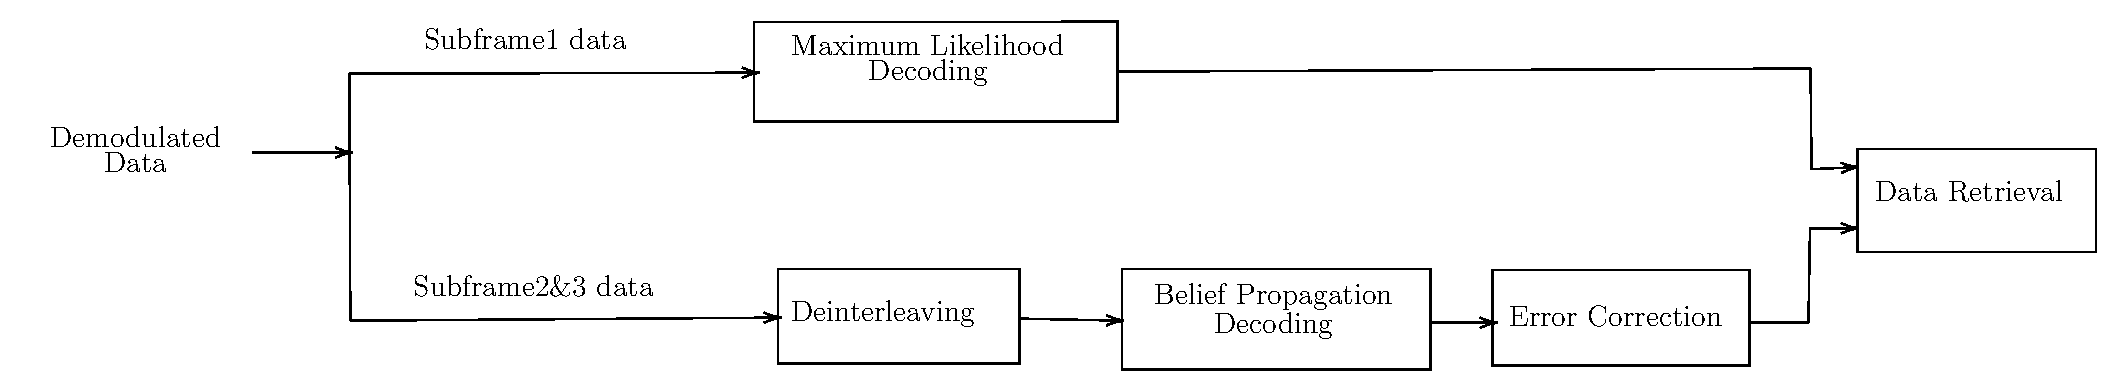
\includegraphics[width=1.2\columnwidth]{figs/decoding_r}
\centering
\captionsetup{justification=centering}
\caption{The Block Level Architecture for Channel decoding}
\label{fig:decoding_r}
\end{figure}
\end{normalsize}


\subsection{Maximum Likelihood Decoding}
The first 52 bits of the frame are a part of subframe 1 and are BCH encoded. To decode these bits, we use a modified version of ML decoding. Before encoding, subframe 1 has 9 bits. These 9 bits give us the TOI (Time of Interval) data. The TOI for NavIC L1 ranges from 1 (000000001) to 400 (110010000). After encoding, SF1 will have 52 symbols. So there will be 400 possible combinations of SF1 before and after encoding. 

So, on the receiving side, we generate these 400 possible codewords and keep them in a lookup table. When a frame is received, the first 52 symbols are separated. The received codeword is compared with every other codeword in the loookup table and the hamming distance is calculated. The codeword in the lookup table which has the least hamming distance with the received codeword is the  corrected codeword (NOTE: Works only if error < 20 bits. This method fails for very noisy channels). The corresponding bit sequence (decoded) can be mapped from the chosen codeword.

\subsection{Deinterleaving}
To reduce the burst error while transimission, the LDPC encoded symbols are interleaved into a 38x46 matrix. Data is written in columns and then, read in rows. So even if there is any burst error, it is spread out. At the receiving side, the matrix is then converted to a regular row of symbols.

\subsection{Belief Propagation}
The basic concept of the algorithm involves message passing. Messages are passed iteratively between adjacent nodes until convergence dictated maximal number of iterations. The nature of the messages involves probabilities or log-likelihoods of probabilities. As nodes receive messages from their nearest neighbors, they improve their estimate regarding received bits. For sufficiently long blocks, with sufficiently long cycles, the algorithm has been shown empirically to perform well.

Variable nodes pass messages that involve the log-likelihood of some bit being 0 or 1 by processing information obtained from other check nodes and the channel whereas check nodes pass messages which involve the log-likelihood of a parity equation is satisfied by processing information obtained from other variable nodes.

For each node of the factor graph, there are two directions of soft information in the form of LLR. The LLR propagated from right to left is denoted as $L_{i,j}$, while that from left to right is denoted as $R_{i,j}$. The decoder employs the so-called processing element (PE), which performs the following LLR estimations with the Min-Sum approximation, so that LLRs are traversed through the factor graph.

BPD is performed on the factor graph by operating the PE from left to right, and from right to left to update L and R, respectively. The final decision is estimated after the completion of all the  iterations. After decoding, CRC is calculated to verify the decoded data.










\chapter{Results}
\section{Acquisition}

\begin{lstlisting}
Acquisition results for PRN ID 2
 Status:True Doppler:680 Delay/Code-Delay:18655/4771.01625
Acquisition results for PRN ID 3
 Status:True Doppler:1480 Delay/Code-Delay:18942/4844.4165
Acquisition results for PRN ID 4
 Status:True Doppler:3960 Delay/Code-Delay:18843/4819.09725
Acquisition results for PRN ID 6
 Status:True Doppler:5000 Delay/Code-Delay:18886/4830.0945
\end{lstlisting}
\newpage
\section{Tracking and Decoding}
\textbf{Result}
\begin{lstlisting}
Tracking and decoding output for PRN ID:2
Subframe1 Before Encoding (9 bits): [1 0 0 0 1 1 1 0 1]
Subframe1 After Encoding (52 Symbols): [0 0 1 0 0 0 1 0 0 0 0 0 0 1 0 0 1 0 0 1 1 0 1 0 0 1 1 1 1 0 1 1 1 0 0 0 0
 1 1 1 1 1 1 1 0 0 0 1 1 1 0 1]
Subframe1 After Receiving (52 Symbols): [1. 1. 0. 1. 1. 1. 0. 1. 1. 1. 1. 1. 1. 0. 1. 1. 0. 1. 1. 0. 0. 1. 0. 1.
 1. 0. 0. 1. 1. 0. 1. 1. 1. 0. 0. 0. 0. 1. 1. 1. 1. 1. 1. 1. 0. 0. 0. 1.
 1. 1. 0. 1.]
Subframe1 After decoding (9 bits): (1, 0, 0, 0, 1, 1, 1, 0, 1)
Subframe2 Before Encoding (600 bits): [1 0 1 1 1 1 0 1 1 0 0 1 1 0 1 0 1 0 1 1 0 0 1 0 1 1 1 0 0 0 0 0 0 0 0 0 0
 0 0 0 1 0 0 1 1 0 1 1 0 0 0 1 0 1 1 0 1 0 1 1 0 1 1 0 0 1 0 0 0 1 1 1 1 1
 0 1 0 1 1 0 0 0 1 1 1 0 1 1 0 1 1 0 .........1 1 1 0 1 1 1 1 1 0 0 1 1 0 1 1 0 1 1 1 1 0 1 1 1 0 1 0 1 0 1 0 0 1 1 0 0
 1 0 1 1 0 1 0 1]
Subframe2 After Encoding (1200 Symbols): [1 1 1 ... 0 1 0]
Subframe2 After Receiving (1200 Symbols): [1. 1. 1. ... 0. 1. 0.]
Subframe2 After decoding (600 bits): [1 0 1 1 1 1 0 1 1 0 0 1 1 0 1 0 1 0 1 1 0 0 1 0 1 1 1 0 0 0 0 0 0 0 0 0 0
 0 0 0 1 0 0 1 1 0 1 1 0 0 0 1 0 1 1 0 1 0 1 1 0 1 1 0 0 1 0 0 0 1 1 1 1 1
 0 1 0 1 1 0 0 0 .........1 1 1 0 1 1 1 1 1 0 0 1 1 0 1 1 0 1 1 1 1 0 1 1 1 0 1 0 1 0 1 0 0 1 1 0 0
 1 0 1 1 0 1 0 1]
Subframe 2 is same before encoding and after decoding: True
             0 <<< remainder
Subframe3 Before Encoding (274 bits): [1 1 1 1 1 0 0 1 0 1 0 1 0 0 0 0 1 0 0 1 0 0 1 0 0 1 0 0 0 1 1 0 0 1 0 1 0
 1 1 1 1 1 1 0 0 0 0 0 1 1 0 1 1 0 1 1 0 1 1 1 1 0 0 0 0 1 1 0 0 1 1 1 0 0
.......... 0 1 0 0 1 0 0 0 0 1 0 1 0 1 0 0 0 0 1 1 1 1 0 0 1 1 0 1 0 0 0 0 0 0 0 1 1
 1 0 1 1 1 0 1 0 0 1 0 1 1 1 1]
Subframe3 After Encoding (548 Symbols): [0 0 1 1 0 0 1 0 0 1 0 0 1 0 1 1 0 1 0 1 1 0 0 0 1 1 1 1 0 0 1 0 0 0 1 1 1
 1 1 0 0 1 0 1 1 1 1 1 0 0 1 1 0 0 0 0 1 0 1 1 1 0 1 0 1 0 1 0 1 1 1 1 1 1
 1 0 1 1 1 0 1 0 1 0 0 1 1 1 1 0 0 1 0 0 1 1 1 1 0 1 1 1 1 0 0 1 1 0 0 0 1
 1 0 0 1 1 0 0 1 1 0 0 0 0 1 0 1 0 1 1 0 0 1
\end{lstlisting}
\begin{normalsize}
\begin{figure}[ht]
\centering
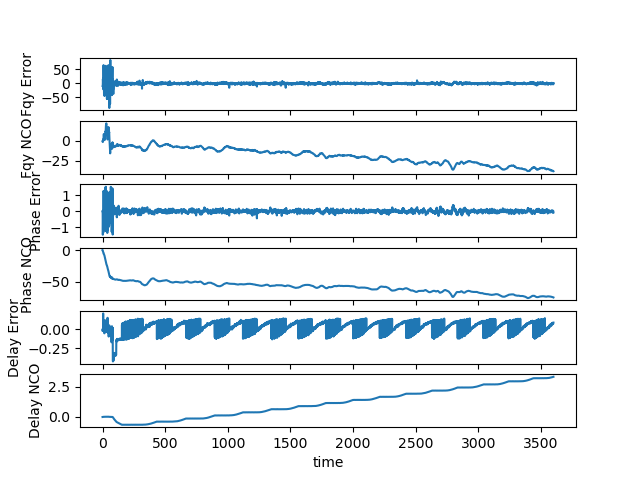
\includegraphics[width=1\columnwidth]{figs/tracking_plot.png}
\centering
\captionsetup{justification=centering}
\caption{Tracking result plot}
\label{fig:tracking_plot}
\end{figure}
\end{normalsize}







\backmatter
\appendix
\chapter{References}
\begin{enumerate}
	\item https://yair-mz.medium.com/decoding-ldpc-codes-with-belief-propagation-43c859f4276d
	
	\item https://www.mdpi.com/2073-8994/14/12/2633
	
	\item https://www.isro.gov.in/media\_isro/pdf/Publications/Vispdf/Pdf2017/\\1a\_messgingicd\_receiver\_incois\_approved\_ver\_1.2.pdf

	\item https://gnss-sdr.org/docs/sp-blocks/acquisition/

	\item https://gnss-sdr.org/docs/sp-blocks/tracking/
   
	\item Elliott D. Kaplan and Christopher J. Hegarty,  Understanding {GPS} {P}rinciples and {A}pplications, $3^{rd}$ edition
\end{enumerate}
\let\cleardoublepage\clearpage  %to remove blank page

%\newpage
%\begin{thebibliography}{00}
%\bibitem{b1} \text{https://www.isro.gov.in/media_isro/pdf/Publications/Vispdf/Pdf2017/1a_messgingicd_receiver_incois_approved_ver_1.2.pdf} 
%\bibitem{b2} \text{https://gnss-sdr.org/docs/sp-blocks/acquisition/}
%\bibitem{b3} \text{https://gnss-sdr.org/docs/sp-blocks/tracking/}
%\bibitem{b4} Elliott D. Kaplan and Christopher J. Hegarty "Understanding GPS Principles and Applications"
%\end{thebibliography}

\latexprintindex
\end{document} 
